\input{/Users/daniel/github/config/preamble.sty}%This is available at github.com/danimalabares/config
\input{/Users/daniel/github/config/thms-eng.sty}%This is available at github.com/danimalabares/config

%\usepackage[style=authortitle-terse,backend=bibtex]{biblatex}
%\addbibresource{/Users/daniel/github/config/bibliography.bib}
\begin{document}
\bibliographystyle{alpha}

\begin{minipage}{\textwidth}
	\begin{minipage}{1\textwidth}
		Math\hfill Daniel González Casanova Azuela
		
		{\small \hfill\href{https://github.com/danimalabares/math}{github.com/danimalabares/math}}
	\end{minipage}
\end{minipage}\vspace{.2cm}\hrule
{\huge math}
\vspace{10pt}

A place to keep track of the things I think I know.

\textbf{Note from May 16.} The part on ag is still very young, recently influenced by Misha's notes \texttt{sergunchik/daniel/other-docs/mag.pdf}. The part on complex geometry is super messy but starting to take shape up to Core concepts subsection and proof of adjunction formula recently posted on Telegram
\tableofcontents
\clearpage
\section{basic math}

\subsection{tensor product}

\begin{defn}[Tensor product by \cite{sea}]\leavevmode
If \(V\) and \(W\) are \(R\)-modules and \(R\) is a ring, I think of the \textit{\textbf{tensor product}} as
\[V\otimes W:=\left\{\sum_{\text{finite} }\lambda_i (v \otimes w)_i, v \in V, w \in W \right\} \Big/ \substack{\begin{array}{c}v \otimes (w_1+w_2)\sim v\otimes w_1+ v\otimes w_2\\ (v_1+v_2) \otimes w \sim(v_1 \otimes w)+(v_2 \otimes w)\\ \lambda(v \otimes w)\sim(\lambda v) \otimes w \sim  v \otimes(\lambda v)\end{array}}\]
More formally, the free \(R\)-module generated by \(V \times W\) (we say this so that things of the kind \(\lambda(v,w)\) make sense) quotiented by the ideal generated by these guys:
\begin{gather*}(v,w_1+w_2)-(v,w_1)-(v,w_2),\\ (v_1+v_2,w)-(v_1,w)-(v_2,w),\\ (\lambda v,w)-\lambda(v,w),\\(v,\lambda w)-\lambda(v,w)\end{gather*}
So that we denote the projection of \((v,w)\) by \(v \otimes w\). Also never forget that the product was defined when you have a product and Vakil has a product…
\begin{thing7}{and I have a product…}[Universal property of product]\leavevmode
It's actually nice to recall that any two objects satisfying the ``every map of such kind factors through a map involving the product"-property, you can construct an isomorphism between them. So the only thing satisfying the product property is the product.
\end{thing7}
\end{defn}
And of course you must understand the construction of tensor product using universal property. Suppose you have a tensor product…

\begin{remark}\leavevmode
Maybe when I think of \(\operatorname{span}\) of some set of symbols I mean the free \(R\)-module generated by the (as many symbols I need)-th product of the place where the symbols live, quotiented by the obvious linearlity relations.
\end{remark}

\begin{remark}\leavevmode
The difference between tensor product and cartesian product is that the latter is not bilinear in addition and scalar multiplication, look:
\begin{align*}
	(v_1,w_1)+(v_2,w_2)&=(v_1+v_2,w_1+w_2),\\
	\lambda(v,w)&=(\lambda v, \lambda w)
\end{align*}
\end{remark}

\begin{thing6}{14.3.6, \cite{sea}}[Tensor algebra constructions]\leavevmode
Let \(M\) be an \(A\)-module. The \textit{\textbf{tensor algebra}} \(T^\bullet(M)\) is just (the direct sum, probably) of \(T^0(M):=A\), \(T^n(M):=\underbrace{M\otimes_A \ldots\otimes_A M}_{n\text{ times} }\).

The \textit{\textbf{symmetric algebra}} \(\operatorname{Sym}^\bullet(M)\) is the quotient of \(T^\bullet (M)\) by the (two-sided) ideal generated by all the elements of the form \(x \otimes y -y \otimes x\). So,
\[\operatorname{Sym}^n(M)=M \otimes \ldots \otimes M \Big/m_1 \otimes \ldots \otimes m_n - m_1' \otimes \ldots \otimes m_n'\]
where \((m_1',\ldots,m_n')\) is a rearrangement of \((m_1,\ldots,m_n)\).

Finally the \textit{\textbf{exterior algebra}} \(\Lambda^{\bullet}(M)\) is defined to be the quotient of \(T^\bullet M\) by the (two-sided) ideal generated by all the elements of the form \(x \otimes x\) for all \(x \in M\). Which implies that \(a \otimes b = -b \otimes a\) (Pf. do \((a+b) \otimes (a+b)\), but only if \(\operatorname{char}\neq 2\) right?) Apparently this gives you that
\[\Lambda^{n}M=\text{quotient of no sé que with a permutation} \]
Anyway I can finally say that if \(\mathcal{F}\) is a locally free rank-\(m\) sheaf, I can define \(T^n \mathcal{F}\), \(\operatorname{Sym}^n\mathcal{F}\) and \(\Lambda^{n}\mathcal{F}\), that will be locally free (exercise, and find their ranks, exercise). And just to conclude for today, the \textit{\textbf{determinant (line) bundle}} is  \(\Lambda^{\operatorname{rk}\mathcal{F}}\mathcal{F}:=\det\mathcal{F}\).
\end{thing6}
So why all this. Because adjunction formula gives you that the canonical bundle of the submanifold is \(K_{\text{ambient mfd}}\otimes_{\mathbb{C}?} \det \mathcal{N}\) where \(\mathcal{N}\) is the normal bundle of the submanifold which is the cokernel sheaf/bundle of the inclusion. So that's that.

\begin{thing7}{Plücker embedding}\leavevmode
It's a way to put Grassman inside a projective space:
\[\operatorname{Gr}(V,k) \hookrightarrow \mathbb{P}\Lambda^{k}V = \operatorname{Gr}(\Lambda^{k}V,1)\]
evidently given by
\[\text{basis } e_1,\ldots,e_k\text{ of \(U \in \operatorname{Gr}(V,k)\)}\longmapsto \operatorname{span}\{e_1 \wedge \ldots \wedge e_k\}\]


\end{thing7}




\subsection{sheaves}

\(\mathfrak{m}_x \subset C^\infty(\mathbb{R}^n)\) is the ideal of smooth functions vanishing at \(x \in \mathbb{R}^n\). In \cite{hart} definition of \textit{\textbf{local ring of \(P\) in \(Y\)}}, which is the ring of germs of regular functions of the variety \(Y\) at the point \(P\), that it is a local ring with maximal ideal \(\mathfrak{m}\), the set of germs of regular functions which vanish at \(P\). The residue field is \(k\).

\begin{exercise}\leavevmode
Show that indeed \(\mathfrak{m}_x\), the ideal of functions vanishing at \(x\), is maximal.
\end{exercise}
\begin{proof}[Solution]\leavevmode
	Suppose that \(\mathfrak{n} \supseteq \mathfrak{m}_x\) is another ideal contained in \(\mathcal{O}_{X,x}\). If \([f] \in \mathfrak{n}\) does not vanish at \(x\), then we can do \([1/f]\) very near  \(x\), giving \([f][1/f] \in \mathfrak{n}\), so that \(\mathfrak{n}=\mathcal{O}_{X,x}\). And if all \([f] \in \mathfrak{n}\) vanish at \(x\), we get \(\mathfrak{n}=\mathfrak{m}_x\).
\end{proof}

\begin{thing6}{Little discussion with GPT}\leavevmode
In differential geometry we have the sheaf \(\mathcal{F}\) of smooth functions. That's like the scalars of some other structure that we build over it: the tangent sheaf, which is defined as derivations on \(\mathcal{F}(U)\). Remember that for any sheaf \(\mathcal{F}\), the elements of \(\mathcal{F}(U)\) are called sections. Yes, the sections of the tangent bundle are vector fields.

(The proof that \(\mathcal{T}_M\), the tangent sheaf, is a locally free \(\mathcal{F}\)-module (and thus a vector bundle) is just showing that \(\partial_i\) are basis of \(\mathcal{F}(U)\).)

The \textbf{tangent bundle} $TM$ of a smooth manifold $M$ is a vector bundle whose dual, the \textbf{cotangent bundle} $T^*M$, is locally generated by differentials $dx^i$.

	In algebraic geometry, we have an analogous structure:

\begin{itemize}
  \item The \textbf{structure sheaf} $\mathcal{O}_X$ assigns to each open set $U \subseteq X$ the ring of regular functions on $U$.
  \item The \textbf{sheaf of Kähler differentials} $\Omega^1_X$ is the analogue of the cotangent bundle: it is an $\mathcal{O}_X$-module generated by formal differentials $df$.
  \item The \textbf{tangent sheaf} $\mathcal{T}_X$ is the dual of $\Omega^1_X$, i.e.,
  \[
  \mathcal{T}_X := \mathcal{H}om_{\mathcal{O}_X}(\Omega^1_X, \mathcal{O}_X),
  \]
  and it corresponds to derivations of the structure sheaf:
  \[
  \mathcal{T}_X(U) = \operatorname{Der}_{\mathbb{K}}(\mathcal{O}_X(U), \mathcal{O}_X(U)).
  \]
  \item These sheaves are \textbf{quasicoherent sheaves}, which generalize vector bundles to the algebraic setting.
\end{itemize}

So, quasicoherent sheaves play the role of vector bundles in algebraic geometry, and in particular, $\mathcal{T}_X$ is the algebraic analogue of the tangent bundle.
\end{thing6}

\section{differential geometry}

\subsection{slice charts and what is ag}

At some point \cite{gri} defines \textit{\textbf{analytic subvariety}} of a complex manifold to be \(V \subset M\) such that \(\forall p \in V\) there is a neighbourhood of \(M\) containing \(p\) where \(V\) looks like the zeros of a single holomorphic function. So that reminds us of:

\begin{thm}[Slice charts for immersion, \cite{les}]\leavevmode
Suppose \(F:M \to N\) is an immersion. Then there are charts \((\varphi,U),(\psi,V)\) such that
\[(\psi \circ F \varphi^{-1})(\vec{x})=(x_1,\ldots,x_m,0,\ldots,0)\]
\end{thm}

\begin{proof}\leavevmode
Just to record that the proof is not \textit{just inverse function theorem}. You do this: pick any random charts \((\overline{\varphi},\overline{U})\) and \((\overline{\psi},\overline{V})\) and consider the Jacobian matrix of \(\hat{F}=\overline{\psi}\circ F \circ \overline{\varphi}^{-1}\). It must have a nonsingular submatrix of rank \(m\) (or of rank \(r\) if you go full constant tank theorem, but that would need some other manipulations…). Then you do:
\begin{enumerate}
\item Reorder the coordinates of the random charts we picked so that the \(\hat{F}\) looks like
	\[\hat{F}=(Q,R)\]
	so that \(dQ\) is nonsingular in the new chart. So you use inverse function theorem to put \(Q\) as a nice local diffeomorphism i.e. a chart. But you are not done:
 \item Figure out how to turn \(Q\) into the identity.
\item Figure out how to turn \(R\) into zero.

	And all that is some manipulations that you'd have to do if you had to teach a course on smooth manifolds, or doing such course (but at this point of the adventure most likely I won't be doing this course right?).
\end{enumerate}
\end{proof}

\subsection{a fact about lie groups and flows}

Not sure where to put this so maybe here for now…

\begin{thing7}{Adjoint representation}\leavevmode
The \textit{\textbf{adjoint representation}} of a Lie group \(G\) is a map \(\operatorname{Ad}:G \to \mathsf{GL}(\mathfrak{g})\) that represents \(G\) as a group of linear automorphisms of its Lie algebra. It is given by \(G \ni a \mapsto (dC_a)_e\), the differential of the conjugation map \(C_a\).
\end{thing7}

\subsubsection*{flow of left-invariant is right multiplication}

Now I know what is a flow: the flow is
\[\varphi^t(p)\]
For every point of the manifold I get the integral curve of a vector field (of course a priori a flow is just a flow but let me just think it's the flow of a vector field). At every point you get a curve.

Now. The thing with the Lie bracket is that when you differentiate the flow you get to the Lie bracket via a formula that is hard to write. So the easy way to write it is:
\[[V,W]=\frac{d}{dt}\Big|_{t=0} \varphi^{-t}_{*,\varphi^t(p)}W_{\varphi^t(p)}\]
and that's it.



Now I will prove in Portuguese that \textbf{the flow of a left-invariant vector field is right-translation}. First I need a claim.

	\begin{claim}\leavevmode
	O fluxo \(\varphi\) de um campo invariante à esquerda \(w\) comuta com a traslação à esquerda, i.e.,
	\[\varphi_t(e)\circ L_h = L_h \circ \varphi_t(e)\qquad \forall t\in \mathbb{R} \forall h \in G.\]
	\end{claim}
	\begin{proof}[Prova da afirmação]\leavevmode
Derivamos de ambos lados. Por um lado,
\begin{align*}
\frac{d}{dt}\Big|_{t=0}\varphi_t(e) \circ L_h=\frac{d}{dt}\Big|_{t=0}\varphi_t(h)&=v_h\end{align*}
Por outro lado,
\[\frac{d}{dt}\Big|_{t=0}L_h \circ \varphi_t(e)=(L_h)_{*,\varphi_t(e)}\frac{d}{dt}\Big|_{t=0}\varphi_t(e)=(L_h)_{*,e}v_e=v_h.\]
Por unicidade das soluções de EDOs, acabou.
	\end{proof}
Então repare:
\[\varphi_t(h)=(\varphi_t\circ L_h)(e)=(L_h \circ \varphi_t)(e)=h\varphi_t(e)=R_{\varphi_t(e)}h,\]
ou seja, qualquer curva integral de \(w\) é simplesmente a curva integral que passa por \(e\) trasladada. \textbf{That's what I wanted to show but there's more:} 

Agora lembre que o colchete de Lie pode ser expressado como
\[[w,v]_e=\frac{d}{dt}\Big|_{t=0}\Big(\varphi_{-t}\Big)_{*,\varphi_t(e)}v_{\varphi_t(e)}.\]
(Onde fixamos o parámetro \(-t\) e deixamos livre o outro para ver \(\varphi_{-t}\) como um difeomorfismo de \(G\).)

Juntando com a discussão anterior obtemos
\[[w,v]_e=\frac{d}{dt}\Big|_{t=0}\Big(R_{\varphi_{-t}(e)}\Big)_{*,\varphi_t(e)}v_{\varphi_t(e)}.\]



\subsection{super technical: how to show vector fields are smooth}

Sometimes we need to show something is smooth and we just say well, everything is smooth so the new thing is also smooth. Here's the formal way to show smoothness for vector fields:

\begin{thing7}{Proposition 8.14}[\cite{les}]\leavevmode
A rough vector field \(X : \to TM\) is smooth iff \(Xf\) is smooth for every \(f\in C^\infty(M)\).
\end{thing7}

\subsection{why I can't understand riemannian geometry}

Unrelated to complex geometry but a breakthrough in my long-standing philosophical search to understand why I can't understand riemannian geometry.

\begin{thing4}{Definition 7.14}[\cite{tud}]\label{def:7.14}\leavevmode
Let \(E\) and \(F\) be vector bundles over a manifold \(M\). An \(\mathbb{R}\)-linear map \(T:\Gamma(E)\longrightarrow \Gamma(F)\) is a \textit{\textbf{point operator}} if whenever two sections \(s,s' \in \Gamma(E)\) coincide at a point \(p\) in \(M\), \(T(s)\) and \(T(s')\) also coincide at \(p\). So:
\[\forall s \in \Gamma(E)\text{ and } \forall  p \in M, \quad s_p=s'_p \implies T(s)_p=T(s')_p\]
and actually (…exercise) that's equivalent to being a \(\mathcal{F}(M)\) linear map, i.e. a \textit{\textbf{tensor}}.

\(T\) is called a \textit{\textbf{local operator}} if whenever two sections coincide in an open set \(U\), so do \(T(s)\) and  \(T(s')\) in that open set.

{\color{2}\bfseries What}\hspace{.5em} Tensors let you do linear algebra globally, and local operators are derivations. Remember that you can take \(F\) to be trivial rank-1 vector bundle and you get \(\Gamma(F)=\)functions so here's all the riemannian geometry.
\end{thing4}

\begin{exercise}\leavevmode
Point operator iff \(\mathcal{F}(M)\)-linear.
\end{exercise}

\begin{proof}[Solution]\leavevmode
(\(\implies\)) You pick a local trivialization of \(E\), so that \(s=\sum s^ie_i\), and then
\(T\left(\sum s^ie_i\right)=\sum s^i T(e_i)\) but since \(s_p=0\), you know that \(s^i=0\) for all \(i\). (\textbf{Rk.}  you have secretly used that point operator \(\implies\) local operator, see \cite{tud}.)

(\(\impliedby\)) You wish that \(T(fs)-fT(s)\) is the zero section of  \(\Gamma(F)\) i.e. that gives the zero vector at all \(p\). Fix \(p\). Define \(s':=fs - f(p)s\). Gives zero at \(p\). So, \(T(s')_p=0\). Then
 \[0=T(s')_p=T(fs-f(p)s)_p=T(fs)_p-f(p)T(s)_p=\Big(T(fs)-fT(s)\Big)_p.\]

\end{proof}

\begin{thing8}{Superpower}\leavevmode
Now you can define tensors pointwise.
\end{thing8}

\begin{thing6}{Opinion}\leavevmode
we should work with bundles
\end{thing6}

\subsection{\(dx^idx^j\) finally explained}

The question is why is \(dx^i  \otimes dx^j\) not defined as an element of any tensor product of vector spaces. But that's  $\mathsf{OK}$ because it is: it's an element of \(T_p^*M\otimes T^*_pM\). But why is not defined like that.

It's defined as the bilinear map \(T_pM \times T_pM\to \mathbb{R}\), \((v,w)\mapsto dx^i(v)dx^j(w)\). And what that has to do with \(T_p ^*M\otimes T_p ^*M\). That by the universal product of tensor product any bilinear map \(T_pM \times T_pM\to \mathbb{R}\) factors uniquely through a map \(T_pM \otimes T_pM \to \mathbb{R}\), i.e. an element of \(\operatorname{Hom}(T_pM \otimes T_pM, \mathbb{R})\). And you probably can prove that \(\operatorname{Hom}(T_pM \otimes T_p M, \mathbb{R})\cong \operatorname{Hom}(T_pM,\mathbb{R})\otimes \operatorname{Hom}(T_pM, \mathbb{R})\overset{\operatorname{def}}{=}T_p ^*M \otimes T^*_pM\).

So: there's a unique guy in the tensor product \(T_p ^*M \otimes T^*_pM\) that corresponds to ``\(dx^i \otimes dx^j\)" defined as a bilinear map \(T_pM \otimes T_pM\to \mathbb{R}\), \((v,w)\mapsto dx^i(v)dx^j(w)\).

And to conclude you just \textit{denote} the symmetrization of \(dx^i \otimes dx^j\), which was previously defined by \(\operatorname{Sym}(dx^i \otimes dx^j)\overset{\operatorname{def}}{=}\frac{1}{2}(dx^i \otimes dx^j +dx^j \otimes dx^i)\), by the symbol \(dx^idx^j\). And to conclude more \textbf{you would prove} that those guys are a basis for \(\operatorname{Sym}^2T_p^*M\overset{\operatorname{def}}{=}(T_p^* M \otimes T_p^*M)/\left<x \otimes y-y \otimes x\right>\). To conclude further bundlize this construction to get \(\operatorname{Sym}^2T^*M\), whose positive-definete sections are the metrics of \(M\).

\begin{thing8}{Trip}\leavevmode
what if that bundle is trivial? You get a global basis for the metric. GPT says: \(\operatorname{Sym}^2T^*M\) is trivial iff \(TM\) is. So in general you don't get global functions \(g_{ij}\) and you compute them locally every time.
\end{thing8}

\subsection{trace}

\begin{thing4}{Proposition 12.10}[\cite{les}]\label{prop:12.10}\leavevmode
If  \(V_1,\ldots,V_k\) are finite-dimensional vector spaces, there is a canonical isomorphism
\[V_1^*  \otimes\ldots \otimes V^*_k \cong \operatorname{Hom}(V_1,\ldots,V_k;\mathbb{R})\]
\end{thing4}
\begin{proof}\leavevmode
You define a bilinear map from \(V^*_1 \times \ldots \times V^*_k \to \mathbb{R}\) that corresponds with the map you want by universal property of tensor product.
\end{proof}

\begin{thing6}{Corollary 12.12}[\cite{les}]\leavevmode
The canonical basis of the tensor product (I wanted this to show that \(dx^i\) are a basis of \(V^* \otimes V^*\)) is given by the last proposition.
\end{thing6}

Anyway the point of contractions is understanding trace. \textit{\textbf{Trace of an endomorphism}} \(T \in \operatorname{End}(V)\) is just
\[\sum_i \left<Te_i,e_i\right>,\qquad \{e_i\}\text{ orthonormal frame} \]
when you have an inner product right? So I showed this is independent of the choice of orthonormal frame. But further, GPT claims this is in fact independent of having a metric and it's actually just the sum of the diagonal entries in any base. So you just need finite dimensional \(V\) and no metric.

And probably I'm not the only guy who ended up reading about trace just because he wanted to understand Ricci. \textit{\textbf{Ricci}} tensor is the trace of the endomorphism  \(R\) when you fix the last two entries and act on the first one. That's it

\subsection{raising and lowering indices}

\[g(X,Y)=g(X^iE_i,Y^j\partial_j)=g_{ij}\varepsilon^i\varepsilon^j(X^jE_k,Y^\ell E_\ell)=g_{ij}X^iY^j\]
Define
\[X^\flat:=X_i\varepsilon^i\]
who's \(X_i\)? The point of of \(\flat\) is that
\[X^\flat =g_{ij}X^i\varepsilon^j\]
(so that you can still eat a vector on the other entry of the metric). So you see
\[X_i=g_{ji}X^j\]
The inverse of the metric matrix exists and is
\[g^{ij}g_{j k}=\delta^i_k\]
Now define
\[\omega^\sharp:=\omega^iE_i\]
so the point is
\[\omega^\sharp=g^{ij}\omega_iE_j\]
(but what that means? \(\omega\) is a form, give you a vector, it's the inverse of the canonical isomorphism). So you see
\[\omega^i=g^{ji}\omega_j\]



\subsection{never forget how to extend riemannian metric to other bundles}

You pick an orthonormal base \(e_i\) of the tangent space and declare that the metric on forms will be the only one that makes the dual base \(\varepsilon_i\) orthonormal. And you check this is well defined. And then you do that for other vector bundles… hmm maybe take one or two more minutes to make sure this is right

\subsection{the pullback bundle and the pullback connection aka all I know}

This is how the pullback connection was born in \cite{au} (and also in \cite{daj} with the caveat that they are using isometric immersions only):

\begin{prop}[Everything I know about connections]\leavevmode
Let \(\nabla\) be a (linear) connection on a vector bundle \(E\) over \(M\). Then, for every \(f:M \to \widetilde{M}\) there exists a unique connection
\[\nabla^f:\mathfrak{X}(\widetilde{M}) \times \Gamma(f^*E) \longrightarrow \Gamma(f^*E)\]
on \(f^*E\) such that
\[{\color{2}\nabla^f_Y(\xi \circ f)=\nabla_{f_* Y}\xi}\]
for all \(Y \in \mathfrak{X}(\widetilde{M})\) and \(\xi \in \Gamma(E)\).
\end{prop}

\begin{proof}\leavevmode
Let me skip the details for now but: suppose it exists. Look how it behaves locally and show uniqueness, meaning that if you had any other connection satisfying the ``all I know" property, they are the same. Then you prove (exercise) that it is indeed a connection. Then you recall that connections are local operators. This somehow shows you that this local uniqueness implies that the connection, if it existed, is globally unique. And you conclude by noticing that yes, you can glue the pieces together to produce a global thing, so the connection does exist.
\end{proof}

Now let's do \cite{mc}. Define \textit{\textbf{connection}} on a bundle \(\zeta\) as a \(\mathbb{C}\)-linear map
\[\nabla:\Gamma(\zeta) \longrightarrow \Gamma(\tau_{\mathbb{C}}^* \otimes \zeta)\]
satisfying \textit{\textbf{Leibniz formula}} 
\[\nabla(fs)=df \otimes s +f \nabla(s)\]
for every \(s \in \Gamma(\zeta)\) and every \(f \in C^\infty(M,\mathbb{C})\).

Right so this definition implies that it's a local operator. In the sense already explained in the section of why I can't understand riemannian geometry. Namely: a local operator of sections of a bundle to sections of another bundle is called \textit{\textbf{local}} if the output section doesn't care about what happens far away. yes, if you take a section and an open set and say well what's the output of this section under the local operator evaluated in this open set and you realise well the output section evaluated at the open set is \textit{completely determined by who is the input section in the open set}.

\begin{quotation}
	``if the section \(s\) vanishes throughout an open set \(U \subset M\) then \(\nabla s\) vanishes thrgoughout \(U\) also. For given \(x \in U\) we can choose a smooth function \(f\) which vanishes outside \(U\) and is identically \(1\) near \(x\). The identity
	\[df \otimes s+ f \nabla s=\nabla(fs)=0\]
evaluated at \(x\), shows that \(\nabla s\) vanishes at \(x\)."	
\end{quotation}
\begin{quotation}
	``Since a connection \(\nabla\) is a local operator, it makes sense to talk about the restriction of \(\nabla\) to an open subset of \(M\). If a colletion of open sets \(U_\alpha\) covers \(M\), then a global connection is uniquely determined by its restrictions to the various \(U_\alpha\)"
\end{quotation}


Then we notice that for any smooth map \(f:M \to \widetilde{M}\) we can pull back functions by precomposing them, and also 1-forms by pullback of 1-forms.

\subsection{the hardest computation of my life so far}
Let \(f:M \to \tilde{M}\) be a map of manifolds and \(p \in \tilde{M}\).  Recall that the differential of \(f\) at \(p\) is a map
\begin{align*}
	f_{*,p}: T_pM &\longrightarrow T_pM \\
	X(p) &\longmapsto f_{*,p}X_p
\end{align*}
defined by
\[(f_{*,p}X_p)g:=X_p(g \circ f)\]
for all \(g \in \mathcal{F}(\tilde{M})\).

Then we have a tensor
\[f_*:\mathfrak{X}(M) \longrightarrow \mathfrak{X}_f\]
that maps a vector field of \(M\) to a section of the pullback bundle \(f^*T\tilde{M}\) that at every point  of \(M\) gives you the vector of \(\tilde{M}\) just defined as \(f_{*,p}X_p\).

There is an exercise that says that the vector fields \(\partial_i\) defined as doing \(\partial_i x^j=\delta_i^j\) are a local basis of sections of \(T\tilde{M}\). But then they are not sections of \(f^*TM\) right so to get sections of pullback bundle you need to put
\[f_* X=X^i(\partial_i \circ f).\]
The question arises:
\[\text{who is } X^i\text{?} \]
The answer reads: on one hand,
\begin{align*}
	(f_*X)_{f(p)}(x^j)&=(X^i \partial_i)_{f(p)}(x^j)=X^i(f(p))(\partial_i)_{f(p)}x^j=X^j(f(p))
\end{align*}
and on the other hand, by definition of differential
\begin{align*}
	(f_*X)_{f(p)}(x^j)&=X_p(x^j\circ f)=X_p(f^j)
\end{align*}
where we denote \(f^j=x^j \circ f\) the coordinate functions of \(f\). So we conclude, for once and for all, that
\[X_{f(p)}(f^j)=X^j(f(p))\]
So we can write
\[f_*X=X(f^i)\partial_i \circ f .\]

\subsection{pullback of torsion}

\begin{exercise}\leavevmode
Mostre que \(T_{\nabla^f}=f^*T\).
\end{exercise}

\begin{proof}[Solution]

\begin{align*}
	T_{\nabla^f}(X,Y)&=\nabla^f_X f_*Y-\nabla^f_Yf_*X-f_*[X,Y]\\
			 &=\nabla^f_XY(f^i)(\partial_i \circ f)-\nabla^f_YX(f^j)(\partial_j\circ f)-f_*[X,Y]\\
			 &=X(Yf^i)(\partial_i \circ f)+Y(f^i)\nabla^f_X(\partial_i \circ f)-Y(Xf^j)(\partial_j\circ f)-Xf^j \nabla^f_Y (\partial_j \circ f)-f_*(XY-YX)\\
			 &=\Big(X(Yf^i)-Y(Xf^i)\Big)(\partial_i \circ f)+Yf^i\nabla^f_X(\partial_i \circ f)-Xf^j\nabla^f_Y(\partial_j \circ f)-(XY-YX)f^i(\partial_i \circ f)\\
			 &=Yf^i \nabla_{f_*X}\partial_i-Xf^j \nabla_{f_*Y}\partial_j\\
&=Yf^iXf^k\nabla_{\partial_k}\partial_i-Xf^jYf^\ell \nabla_{\partial_\ell}\partial_j\\
&=Yf^iXf^k \nabla_{\partial_k}\partial_i-Xf^kYf^i \nabla_{\partial_i}\partial_k\\
&=Yf^iXf^k(\nabla_{\partial_k}\partial_i-\nabla_{\partial_i}\partial_k)\\
&=Yf^iXf^k(\nabla_{\partial_k}\partial_i-\nabla_{\partial_i}\partial_k-[\partial_k,\partial_i])\\
&=Yf^iXf^kT(\partial_k,\partial_i)\\
&=T(f_*X,f_*Y)\\
&=(f^*T)(X,Y)
\end{align*}
\end{proof}

\subsection{fundamental property of isometric immersions}

\begin{thing6}{Exercício L3.2}[Imersões isométricas]\label{exer:L3.2}\leavevmode
Seja \(f:M \to \overline{M}\) uma imersão isométrica. Sejam \(\nabla\) a conexão de Leci-Civita de \(M\) e \(\overline{\nabla}\) a conexão de Levi-Civita de \(\overline{M}\).
\begin{enumerate}[label=(\alph*)]
\item Let \(f:M^n \to \widetilde{M}^m\) be an isometric immersion and let \(\widetilde{\nabla}\) denote the connection on \(f^*T \widetilde{M}\) induced by the Levi-Civita connection of \(\widetilde{M}\). Verify that
	\[\nabla_XY=f^{-1}_*\left(\widetilde{\nabla}_X f_*Y\right)^\top\]
defines a compatible torsion-free connection on \(TM\), which itherefore coincides with the Levi-Civita connection of \(M\).	

\item  (Reformulation of (a).) Mostre que
	\[f_*(\nabla_XY)=\left(\overline{\nabla}^f_Xf_*Y\right)_{TM}\]
e que essa igualdade determina \(\nabla\) em função de \(\overline{\nabla}\). Aqui, para \(W \in T_{f(p)}\overline{M}\), \(W_{TM}\) denota a sua projeção ortogonal ao subespaço \(f_*(T_pM) \subset T_{f(p)}\overline{M}\).
\item Seja \(c\) uma curva suave em \(M\). Mostre que para todo \(Y \in \mathfrak{X}_c\) vale
	\[f_*\nabla^c_{\frac{d}{dt}}Y=\left(\nabla^{f \circ c}_{\frac{d}{dt}}f_*Y\right)_{TM} \]
\item Seja \(\gamma:I \to M\) uma curva suave parametrizada pelo comprimento de arco. Mostre que \(\gamma\) é uma geodésica de \(M\) se, e somente se, sua aceleração em \(\overline{M}\) é perpendicular à variedade \(M\), i.e.,
	\[\overline{\nabla}^{f \circ \gamma}_{\frac{d}{dt}\Big|_{t}}(f \circ \gamma)' \perp f_*(T_{\gamma(t)}M)\]
	para todo \(t \in I\).
\end{enumerate}
\end{thing6}

\begin{proof}[Solução]\leavevmode
\begin{enumerate}[label=(\alph*)]
\item Nos han enseñado que esto se hace así (como dice la version de \cite{daj}): defina
	\[D: \mathfrak{X}(M)\times \mathfrak{X}(M) \longrightarrow \mathfrak{X}(M)\]
una conexión random pero satisfaciendo que
\[f_*(D_XY) = \left(\widetilde{\nabla}_X^f f_*Y\right)^\top\]
. Afirmamos que \(D\) es métrica y simétrica, o sea, \(D=\nabla\) y se acabó. (Que básicamente es el ``lema de simetría y compatibilidad".)
\begin{itemize}
\item \textbf{(Métrica.)} Se me antoja empezar con \(X\left<Y,Z\right>=\) pero ahí no sé que poner. (Puedo poner \(\nabla\) pero eso no sirve de nada.) Entonces mejor aplico \(f_*\), después de pensarlo me doy cuenta de que \(f_*Y\) y \(f_*Z\) son secciones de \(f^*\widetilde{M}\), o sea vectores en \(T\widetilde{M}\) pero como funciones están definidas em \(M\)! Acaba que lo que único que tiene sentido escribir es:
\begin{align*}
X\left<f_*Y,f_*Z\right>&=\left<\widetilde{\nabla}^f_Xf_*Y,f_*Z\right>+\left<f_*Y,\widetilde{\nabla}^f_Xf_*Z\right>
\end{align*}
\(\mathsf{OK}\) pero… eso es cierto? Bueno, lo que sabemos es que:
\begin{align*}
\left<\left( \widetilde{\nabla}^f_Xf_*Y\right)^\top,f_*Z\right>+\left<f_*Y,\left(\widetilde{\nabla}^f_Xf_*Z\right)^\top\right>&=\left<f_*(D_XY),f_*Z\right>+\left<f_*Y,f_*(D_XZ)\right>
\end{align*}



Ah, entonces eso es lo que hay que probar justamente. Me fijo en el lado izquierdo y digo bueno en cada punto, como \(f\) es isometría local,
\[\left<f_{*,p}Y(p),f_{*,p}Z(p)\right>_{f(p)}=\left<Y(p),Z(p)\right>_{p}\]
y como es un tensor escribo nomás
\[\left<f_*Y,f_*Z\right>=\left<Y,Z\right>\]
Y eso sí,
\[\left<Y,Z\right>=\left<\nabla_XY,Z\right>+\left<Y,\nabla_XZ\right>\]
No sé qué hacer con esos campos pero en campos coordenados sí, porque la base de  \(T_p\widetilde{M}\) es \(\partial_i\), pero eso no es una base del fibrado pullback, la que sí es base del fibrado pullback es \(\partial_i \circ f\). Ah entonces
\begin{align*}
\left<\widetilde{\nabla}_X^f \partial_i \circ f,\partial_i \circ f\right>+\left<\partial_j \circ f,\widetilde{\nabla}_X^f \partial_j \circ f\right>&= \left<\tilde{\nabla}_{f_*X}\partial_i,\partial_j\right>+\left<\partial_i,\widetilde{\nabla}_{f_* X}\partial_j\right>\\
&=f_*X\left<\partial_i, \partial_j\right>\\
&=X\left<\partial_i \circ f,\partial_j \circ f\right>
\end{align*}
\end{itemize}

\end{enumerate}
\end{proof}




\subsection{riemannian submersion finally and also riemannian immersion}

For any smooth manifold submersion \(\pi:\widetilde{M}\to M\) there is always a bundle isomorphism I love:
\[\pi^*TM \oplus \kappa\cong T\widetilde{M}\]
where \(\kappa\) is the bundle whose fiber is the kernel of \(\pi_*\), and is also called the \textit{\textbf{vertical bundle}}, and there's no magic in proving that isomorphism, you can do it all the time.

 But we call \(\pi\) a \textit{\textbf{riemannian submersion}} only when \(\pi^*TM\) is isometric to \(TM\), meaning we had put metrics on \(\widetilde{M}\) and \(M\) a priori. And that's it. It just took me 4328 days to understand that. (Definition given in the homework sheet is very different from that; milnor won't talk about this.)

Now riemannian immersion. That is, isometric immersion. So initially \cite{mc} defines for any subbundle \(\xi \subset \eta\) over a riemannian manifold the  \textit{\textbf{orthogonal complement bundle}} \(\xi^\perp\) using the riemannian metric. Then he says well this is called \textit{\textbf{normal bundle}} when you are a submanifold and then says well actually this works for any immersion \(f:M \to \widetilde{M}\) and finally concludes in coro. 3.5 that
\[f^*T\widetilde{M} \cong TM \oplus  \nu\]
Then you get problem 3-B: for vector bundles \(\xi \subset \eta\) define the \textit{\textbf{quotient bundle}} \(\eta/\xi\) and prove it's locally trivial. If \(\eta\) has a Euclidean (riemannian) metric, \(\xi^\perp \cong \eta/\xi\). So I guess that the subtlety is that when everything is riemannian you get that these isomorphisms become isometries of bundles. That is to say: I think that an \textit{\textbf{isometric immersion}} is when \(f^* T \widetilde{M}|_{M}\cong TM\) isometrically which is just that pullback metric is the metric. right

(And also because I was told by V. Ramos that we can define normal bundle equivalently as the quotient bundle \(T\widetilde{M}/TM\) and as the orthogonal complement of \(TM\) wrt any riemannian metric we choose on \(\widetilde{M}\) for means of saying what is the normal bundle. But of course this means that \(T\widetilde{M}/TM\) is \textit{isomorphic} to \(TM^\perp\) and not necessarily \textit{isometric}, as the definition of riemannian submersion says.)

Final resolution: that inclusions put \(M\) inside \(\widetilde{M}\), but submersions don't put \(M\) inside \(\widetilde{M}\): the quotient is a weird thing that might not live in the larger manifold. But strangely enough, its tangent bundle does. So I asked GPT: what if we integrate the bundle and we find a copy of \(M\) inside \(\widetilde{M}\)? And the answer is not always, you need integrability, sometimes yes.

\subsection{volume form at once}

Never forget how to change variables like a pro: if \(F:U \to F(U)\) is a diffeomorphism,
\[\int_U F^*\omega=\int_{F(U)}\omega.\]
Now you need to know what is the pullback of top forms. 

\begin{thing7}{Pullback of top-forms}\leavevmode
A diffeomorphism \(\varphi:M \to \widetilde M\), which is a diffeomorphism, it must be a diffeomorphism for these things to exist. (But eventually you want to integrate the surface, the world-sheet, in the ambient space \(X\) but easy.) So it's a diffeomorphism and you take local charts \((x_1,\ldots,x_n)\) of \(M\) and \((y_1,\ldots,y_n)\) of \(\widetilde{M}\).

You get a top-form on the chart \(\widetilde{U}\) of \(\widetilde{M}\) called \(dy_1\wedge\ldots \wedge dy_n\). If you pull it back, you get a new top-form on \(U\) called \(\varphi^*(dy_1\wedge\ldots \wedge dy_n\). Being top-forms, you know there's a function so that the new guy is that function times \(dx_1\wedge\ldots\wedge dx_n\), which is also a top-form on \(U\). \textbf{Who's the function?} The function is the determinant of the jacobian matrix of your map:
\[\varphi^*(dy_1\wedge\ldots\wedge dy_n)=\det D\varphi dx_1\wedge\ldots\wedge dx_n.\]
\end{thing7}

Now you need to know how to deal with those things.
\begin{thing7}{Fact about top-forms}\leavevmode
Top-forms are determinants.
\[\varepsilon_1 \wedge \ldots \wedge \varepsilon_n(E_1,\ldots,E_n)=\det \varepsilon_i(E_j)\]
where \(\varepsilon_i\) are any 1-forms and \(E_i\) are any vector fields. (Notation is reminiscent of orthonormal frames but this is very general.) Note that for lower-degree forms there is also determinant-like formulas of the kind sum over permutations some products, they are not very nice and hopefully you don't need to use them anytime soon.
\end{thing7}

Now you need to know what is the pullback of top forms. 

Now you want to know what happens in the case of the Volume forms. The volume forms can be exactly the guys from the last Fact if you happen to have orthonormal coordinates. So you get:
\[\varphi^*\operatorname{Vol}_{\widetilde{M}}=\det D\varphi \operatorname{Vol}_M.\]

Which is great. So you can integrate:
\[\int_M \varphi^*\operatorname{Vol}_{\widetilde{V}}=\int_M \det D\varphi \operatorname{Vol}_M\]
And if \(\varphi\) is an isometry the determinant of its differential is… 1. \textbf{Why}. Because \(d \varphi\) is given the matrix whose columns are the images of an orthonormal frame, and these form an orthonormal frame because \(f\) preserves the metric, so the determinant of an orthonormal frame is 1.  So volumes coincide. Yiipa!


\subsection{exponential map and geodesics locally}

Qué es una geodésica localmente?
\[\operatorname{exp}_p(tv)=\gamma(t)\]

Cómo inventas una geodésica que va \(q\) a \(q'\) dentro de la bola \(B_\varepsilon(p)\subset M\)?
\[\underbrace{\operatorname{exp}_q^{-1}q'}_{\substack{\text{vector que}  \\\text{apunta hacia \(q'\)}\\\text{desde \(q\)}   }} \in T_q M\]
Y ahora geodegiquizas:
\[\operatorname{exp}_q\Big(t\operatorname{exp}_q^{-1}q'\Big):=\gamma_{q,q'}(t)\]

\subsection{first variation formula}

This is actually an exercise:

\begin{thing4}{Exercício 8}[Curvas minimizantes]\label{exer:8}\leavevmode
Seja \(\gamma\) uma curva suave por partes parametrizada por comprimento de arco (this is important, velocity is 1) conectando \(p\) a \(q\). Mostre que se \(d(p,q)=\ell(\gamma)\) então \(\gamma\) é uma geodésica.
\end{thing4}

We shall use the \textit{\textbf{first variation formula}} which in short says
\[S'(0)=-\int_a^b \left<V,\gamma''\right>dt.\]
Explanation. Consider a \textit{\textbf{variation}} of \(\gamma\), which is like a homotopy:
\begin{align*}
	\Gamma: (a,b)\times(-\varepsilon,\varepsilon) &\longrightarrow M \\
	\Gamma(t,s) &=\gamma(t)+sV(\gamma(t))
\end{align*}
where \(V \in \mathfrak{X}_\gamma\) is a vector field along \(\gamma\) called the \textit{\textbf{variation field}}, and it has to vanish on the endpoints. Then there's the \textit{\textbf{length functional}} 
\[S(s):=\ell(\Gamma(t,s))=\int_a^b|\nabla_{\frac{d}{dt}}\Gamma(t,s)|dt.\]
Because \(\gamma=\Gamma(t,0)\) is minimizing, we know that \(S'(0)=0\). Then we compute that and hope that it will say \(\gamma''=0\).
\begin{align*}
S'(0)&=\int_a^b\frac{d}{ds}\Big|_{s=0}\left<\nabla_t\Gamma(t,s),\nabla_t\Gamma(t,s)\right>^{1/2}dt\\
&=\int_a^b \frac{\cancel{2}}{\cancel{2}\cancelto{1}{\left|\Gamma(s,t)\right|}}\left<\nabla_s \nabla_t\Gamma(t,s),\nabla_t\Gamma(t,s)\right>dt\\
&\overset{\substack{\text{symmetry}  \\ \text{lemma} }}{=}\int_a^b\left<\nabla_t\underbrace{\nabla_s\Gamma(t,s)}_{=V},\nabla_t\Gamma(t,s)\right>dt\\
&=\int_a^b\frac{d}{dt}\Big|_{t=0}\left<V,\nabla_t\Gamma(t,s)\right>-\int_a^b\left<V,\underbrace{\nabla_t\nabla_t\Gamma(t,s)}_{\gamma''}\right>dt
\end{align*}
and the first one vanished out fundamental theorem of calculus and the fact that \(V\) is zero on the endpoints.

So we get that if \(\gamma\) minimizes distance, this integral is zero for any variation of \(\gamma\).

\begin{thing8}{Remarks}\leavevmode
\begin{itemize}
\item Symmetry lemma just follows from commutativity of partial derivatives in \(\mathbb{R}^{n}\). Florit used pullback connection and \cite{ler} used Christoffel symbols.
\item The true version of the variation formula admits that \(\Gamma\) is only piecewise smooth. The formula becomes less nice and the proof a little more involved, I won't do it, but something nice comes out of that: the fact that you realise that geodesics can't have corners because:
	\begin{figure}[H]
		\centering
		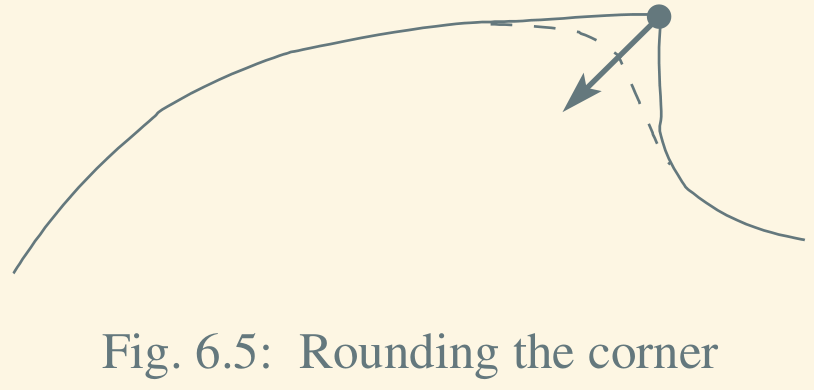
\includegraphics[width=0.3\textwidth]{fig3}
	\end{figure}
	so it would be nice to understand that precisely but \(\mathsf{OK}\).
\end{itemize}
\end{thing8}



\subsection{jacobi field}

Just because I finally understood something about Jacobi field. A geodesic is given by \(\gamma_v(t)=\operatorname{exp}_p(tv)\) where \(p=\gamma(0)\) and \(v=\gamma'(0)\). Then choose a vector \(w \in T_pM\) and consider these lines:
\begin{figure}[H]
	\centering
	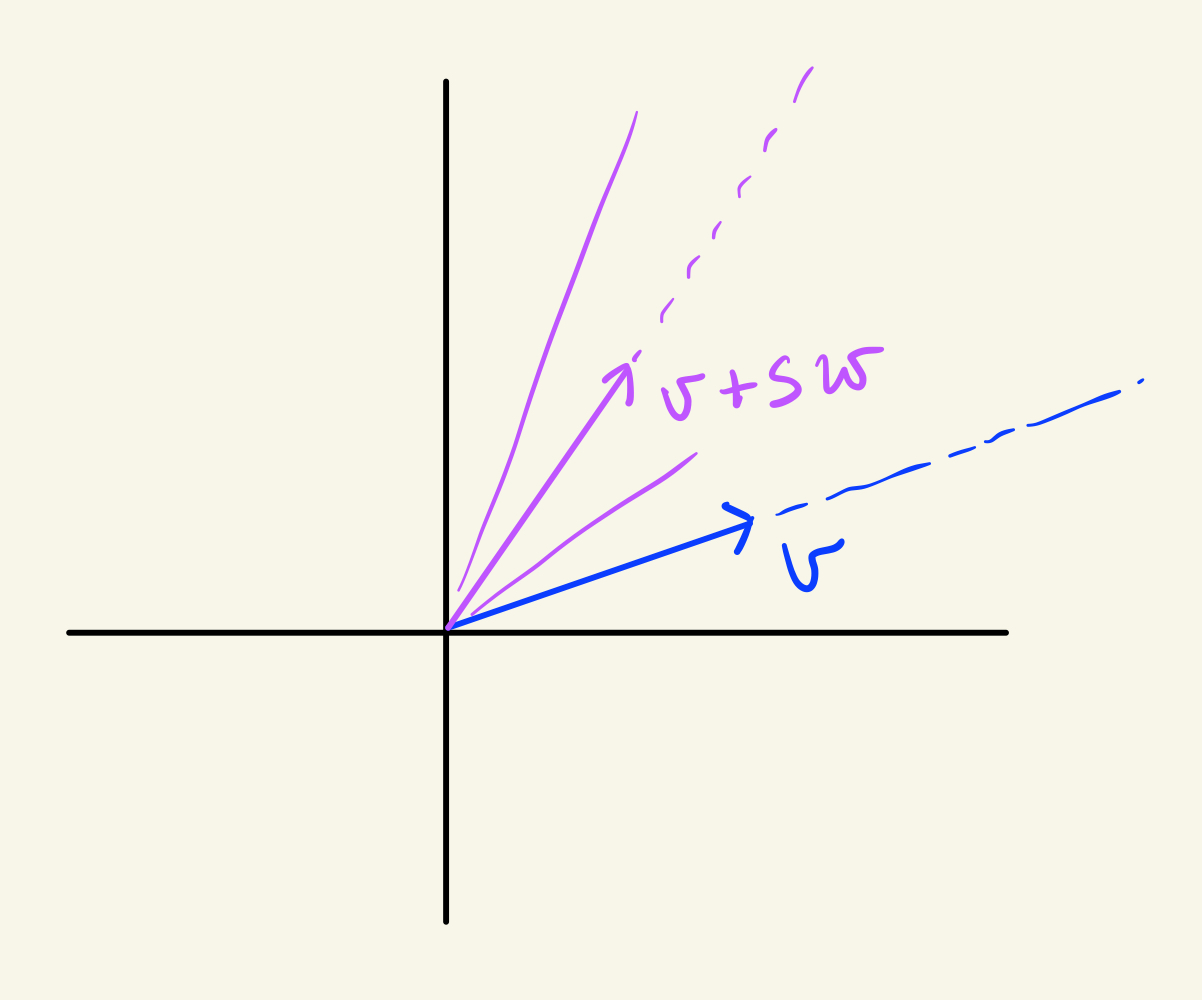
\includegraphics[width=0.4\textwidth]{fig2}
\end{figure}
Then taking \(\operatorname{exp}\) maps them to some geodesics. Then the \textit{\textbf{Jacobi field in this case}} is given by differentiating with respect to \(s\) along the curve \(tv\):
\begin{align*}\nabla_s \gamma_{v+sw}(t)&=\nabla_s \operatorname{exp}_p(t(v+sw))=d_{tv}\operatorname{exp}_p\cdot \frac{d}{ds}\Big(t(v+sw)\Big)\\&=d_{tv}\operatorname{exp}_p(tw).\end{align*}
And that's it.

\subsection{riccati equation}

Take any point and any tangent vector at that point. Take the geodesic and take the geodesic sphere of raduis say \(\varepsilon\) with center in the point. It's a hypersurface. Normal vectors are all multiples of the unit normal vector. But who's that, the unit normal? Ah, it's the speed of the geodesic. So? The normal derivative of any vector field tangent to the sphere w.r.t. the unit normal is…
\begin{align*}
0&=X\left<\nu,\nu\right>=2\left<\nabla^\perp_X \nu,\nu\right>
\end{align*}
that is, normal derivative of \(\nu\) w.r.t. \(X\) is perpendicular to \(\nu\), BUT normal derivative is normal so it's actually a multiple of \(\nu\), which makes \(\nu\) have norm zero or else \(\nabla^\perp_X \nu=0\).

Great! Now you take a variation \(f(s,t)\) which I think is our beloved Jacobi variation
\[d_{tv}\operatorname{exp}_p(sw)\]
and do
\begin{align*}
\nabla &= \ldots=J
\end{align*}
that is,
\[A(J)=J'\]
differentiate that or \(\overline{J}\) to obtain
\[A'+A^2+R_{\gamma'}=0\]





\section{algebraic geometry}
\vspace{1em}
\begin{quotation}
so afraid of this

\hfill ---dani
\end{quotation}
\vspace{2em}
\subsection{algebraic variety}

An \textit{\textbf{algebraic variety}} is a compact topological space equipped with a ring of sheaves which is locally isomorphic to an affine variety with its sheaf of regular functions and Zariski topology.

Amazing! An affine variety sure it's \(Z\), the solution set of some polynomial equations on \(\mathbb{C}^n\) equipped with the ring of algebraic functions, which are the restrictions of polynomial functions to \(Z\). Zariski topology sure, closed sets are also solution sets of algebraic equations.

But what is the sheaf of regular functions? Pick \(U \subset M\) a Zariski open subset that is a union of open Zariski subsets, \(U=\bigcup U_\alpha\). A function on \(U\) is \textit{\textbf{regular}} if it is regular on \(U_\alpha\).

So? What is an algebraic variety? It is a compact topological space with a sheaf that is locally isomorphic to an affine variety \textbf{meaning} that 

\begin{tcolorbox}[colback=white,colframe=black,boxrule=0.5pt,sharp corners]
every open set with the sheaf restricted to the open set is isomorphic as a ringed space to an affine variety equipped with the sheaf of regular functions.
\end{tcolorbox}

\subsection{ag is dg and dg is ag}

This is Misha's construction of smooth manifolds using sheaves. I worked on this construction during norther-hemisphere winter 2024. See \href{https://github.com/danimalabares/dt}{github.com/danimalabares/dt}.

\begin{thing3}{Definition 2.10}\leavevmode
	A \textit{\textbf{ringed space}} $(M,\mathcal{F})$ is a topological space equipped with a sheaf of functions. A \textit{\textbf{morphism}} $(M,\mathcal{F}) \xrightarrow{\psi}(N,\mathcal{F})$ of ringed spaces is a continuous map $M \xrightarrow{\psi}N$ such that, for every open subset $U \subset N$ and every function $f \in \mathcal{F}'(U)$, the function $f \circ \Psi$ belongs to the ring $\mathcal{F}(\Psi^{-1}(U))$. An \textit{\textbf{isomorphism}} of ringed spaces is a homeomorphism $\Psi$ such that $\Psi$ and $\Psi^{-1}$ are morphisms of ringed spaces.
\end{thing3}

\begin{thing5}{Remark 2.6}\leavevmode
	Usually the term ``ringed space" stands for a more general concept, where the ``sheaf of functions" is an abstract ``sheaf of rings", not necesarily a subsheaf in the sheaf of all functions on  $M$. The above definition is simpler, but less standard.
\end{thing5}

\begin{thing4}{Exercise 2.16}\label{exer:2.16}\leavevmode
Let $M, N$ be open subsets in $\mathbb{R}^n$ and let  $\Psi:M \to N$ be a smooth map. Show that $\Psi$ defines a morphism of spaces ringed by smooth functions.
\end{thing4}

\begin{proof}[Solution]\leavevmode
Let $\mathcal{F}$ be the sheaf of smooth functions on $M$ and  $\mathcal{F}'$ on $N$. Choose an open subset $U\subset M$ and $f \in \mathcal{F}'(U)$. Since $\Psi$ is smooth and composition of smooth functions is smooth, $f \circ \Psi$ is a smooth map.
\end{proof}

\begin{thing4}{Exercise 2.17}\label{exer:2.17}\leavevmode
Let $M$ be a smooth manifold of some class and let $\mathcal{F}$ be the space of functions of this class. Show that $\mathcal{F}$ is a sheaf.
\end{thing4}

\begin{proof}[Solution]\leavevmode
Let $U$ be an open set of $M$. To show $\mathcal{F}$ is a presheaf notice that the restriction of a function of class $C^i$ to an open subset is also of class $C^i$. To show $\mathcal{F}$ is a sheaf fix an open set $U \subset M$, an open cover $\{U_j\}$ of $U$, and a collection of functions $f_j \in \mathcal{F}(U_j)$. As in Exercise \hyperref[exer:2.14]{2.14}, differentiability class $C^i$ is a local condition and thus gluing the $f_j$ produces a $C^i$ function on $U$.
\end{proof}

\begin{thing4}{Exercise 2.18}[Smooth sheaf!!!!]\label{exer:2.18}\leavevmode
Let $M$ be a topological manifold, and let $(U_i,\varphi_i)$ and $(V_j,\psi_j)$ be smooth structures on $M$. Show that these structures are equivalent if and only if the corresponding sheaves of smooth functions coincide.
\end{thing4}

\begin{proof}[Solution]\leavevmode
First let's clarify what is the sheaf of smooth functions associated to a smooth structure. Let $U \subset M$ be open.  The ring $\mathcal{F}(U)$ associated to the atlas $(U_i,\varphi_i)$ consists of functions $f:U \to \mathbb{R}$ such that $f \circ \varphi_i^{-1}$ is smooth for all $i$.

Also recall that equivalence of smooth structures means that there is a common refinement of the covers $\{U_i\}$ and $\{V_j\}$ such that $\psi_k\circ \varphi_k^{-1}$ is smooth for all $k$ indexing the refinement.

$(\implies )$ Suppose that $(U_i,\varphi_i)$ and $(V_j,\psi_j)$ are equivalent. The corresponding sheaves $\mathcal{F}_1$ and $\mathcal{F}_2$ coincide because functions are smooth with respect to one atlas iff they are smooth with respect to the other. Indeed: fix $U \subset M$ open and a function $f \in\mathcal{F}_1(U)$. Then $f \in \mathcal{F}_2(U)$ since
\[f \circ \psi^{-1}_j=f \circ (\varphi_i^{-1}\circ \varphi)\circ\psi_j^{-1}=(f \circ \varphi_i^{-1})\circ (\varphi\circ\psi_j^{-1}).\]
which is smooth.

$(\impliedby)$. Suppose that $\mathcal{F}_1$ and $\mathcal{F}_2$ coincide. Let $W_{ij}:=U_i \cap V_j$ be a common refinement of $\{U_i\}$ and $\{V_j\}$. Set $\varphi_{ij}=\varphi_i|_{W_{ij}}$ and $\psi_{ij}=\psi_j|_{W_{ij}}$. \textbf{We must show that $\psi_{ij}\circ \varphi_{ij}^{-1}$ is smooth.} Idea: to use the fact that the sheaves coincide we can use the coordinate functions of the charts, which are real-valued functions and thus must be elements of the sheaves.

Notice that $\psi_{ij}$ consists of $n:=\dim M$ coordinate functions  $\psi_{ij}^\ell:M \to \mathbb{R}$. Each of this functions is smooth with respect to the smooth structure $(V_j,\psi_j)$ since it is the projection onto the $\ell$-th coordinate, that is,
\[\psi_{ij}^\ell \circ \psi_{ij}^{-1}(x_1,\ldots,x_\ell,\ldots,x_n)=x_\ell.\]
Since the sheaf of smooth functions with respect to the smooth structure $(U_i,\varphi_i)$ is the same, $\psi_{ij}^\ell \circ \varphi_{ij}$ must be smooth for all $\ell$, making $\psi_{ij}\circ \varphi_{ij}^{-1}$ smooth.
\end{proof}

\begin{thing5}{Remark 2.7}\label{rk:2.7}\leavevmode
This exercise implies that the following definition is equivalent to the one stated earlier.
\end{thing5}

\begin{thing3}{Definition 2.11}\label{def:2.11}\leavevmode
	Let $(M,\mathcal{F})$ be a topological manifold equipped with a sheaf of functions. It is said to be a \textit{\textbf{smooth manifold of class}} $C^\infty$ or  $C^i$ if every point in $(M,\mathcal{F})$ has an open neighbourhood isomorphic to the ringed space $(\mathbb{R}^n, \mathcal{F}')$, wherre $\mathcal{F}'$ is a ring of functions on $\mathbb{R}^n$ of this class.
\end{thing3}

\begin{thing3}{Definition 2.12}\leavevmode
A \textit{\textbf{coordinate system}} on an open subset $U$ of a manifold $(M,\mathcal{F})$ is an isomorphism between $(U,\mathcal{F})$ and an open subset in $(\mathbb{R}^n,\mathcal{F}')$, where $\mathcal{F}'$ are functions of the same class on $\mathbb{R}^n$.
\end{thing3}

\begin{thing5}{Remark 2.8}\leavevmode
In order to avoid complicated notation, from now on we assume that all manifolds are Hausdorff and smooth (of class $C^\infty)$. The case of other differentiability classes can be considered in the same manner.
\end{thing5}

\begin{thing4}{Exercise 2.19}[!]\label{exer:2.19}\leavevmode
Let $(M,\mathcal{F})$ and $(N,\mathcal{F}')$ be manifolds and let $\Psi:M \to N$ be a continuous map. Show that the following conditions are equivalent.
\begin{enumerate}[label=(\roman*)]
\item In local coordinates $\Psi$ is given by a smooth map
\item $\Psi$ is a morphism of ringes spaces.
\end{enumerate}
\end{thing4}

\begin{proof}[Solution]\leavevmode
(i)$\implies $(ii). Suppose that in local coordinates $\Psi$ is given by a smooth map. Showing that $\Psi$ is a morphism of ringed is spaces is to show that for any open set $U \subset N$ and smooth function $f \in\mathcal{F}'(U)$, the function $f \circ \Psi$ is smooth on $\Psi^{-1}(U)$. The latter means that for each chart $(U_i,\varphi_i)$ of $\Psi^{-1}(U)$, the composition  $(f \circ\Psi)\circ \varphi_i^{-1}$ is smooth.

\[\begin{tikzcd}[column sep=large,row sep=large]
	\mathbb{R}&M\arrow[r,"\Psi"]\arrow[d,swap,"\varphi"]\arrow[l,swap,"f \circ \Psi",bend right]& N\arrow[d,"\psi"]\arrow[r,"f",bend left]&\mathbb{R}\\
	&\mathbb{R}^m\arrow[r,"\psi\circ\Psi\circ \varphi^{-1}",swap]&\mathbb{R}^n
\end{tikzcd}\]
The definition of $f$ being smooth in $U$ is that  $f \circ \psi^{-1}_j$ is smooth in any chart $(V_j,\psi_j)$. Starting from $\mathbb{R}^m$, we can go right instead of up to see that
\[(f \circ \Psi)\circ \varphi^{-1}=(f \circ \psi^{-1}) \circ (\psi \circ \Psi \circ\varphi^{-1}),\]
which is smooth.

{\color{2}Misha: this is almost trivial, should be easier.}

(ii)$\implies $ (i). Now suppose that the pullback of smooth functions (defined on open sets) by $\Psi$ is smooth. Choose the coordinate functions $\psi^\ell$ of a local chart $\psi$. Then $\psi^\ell \circ \Psi \circ \varphi^{-1}$ is smooth for all $\ell$ and for any local chart $(U,\varphi)$ of $M$, making $\psi \circ \Psi \circ \varphi^{-1}$ smooth as well.

{\color{2}Misha: and this shouldn't be that easy.}
\end{proof}

\begin{thing5}{Remark 2.9}\label{rk:2.9}\leavevmode
An isomorphism of smooth manifolds is called a \textit{\textbf{diffeomorphism}}. As follows from this exercise, a diffeomorphism is a homeomorphism that maps smooth functions onto smooth ones. {\color{14}Because the inverse map pulls back smooth functions to smooth ones, so the map itself maps smooth functions to smooth ones.}
\end{thing5}

\subsection{segre}

Here's a summary written by ChatGPT after we discussed Segre embedding:

The Segre embedding provides a way to map the product of two projective spaces into a higher-dimensional projective space. Let \( V \) and \( W \) be two vector spaces of dimension \( n+1 \) and \( m+1 \), respectively. The Segre embedding embeds the product \( \mathbb{P}(V) \times \mathbb{P}(W) \) into \( \mathbb{P}(V \otimes W) \).

\subsubsection*{misha's approach}

A tensor \(\alpha \in V \otimes W\) is called \textit{\textbf{decomposable}} if  \(\alpha=x \otimes y \) for some \(x \in V\), \(y \in W\). (That is, it is only one summand---elements of tensor product are finite sums of thing of that kind.) \textbf{Claim.} A tensor \(\alpha \in V \otimes W\) is decomposable iff the rank of the corresponding map \(V^* \to W\) is \(\leq 1\), where rank is dimension of image.

Cool but what's the corresponding map? It's \(V \otimes W =\operatorname{Hom}(V^*,W)\) defined like this: for a tensor \(\alpha^{ij}v_i \otimes w_j\) define \(\varphi \mapsto \alpha^{ij}\varphi(v_i)w_j\). To see injective: if the image is zero then \(\varphi(v_i)=0\) for all \(i\), so \(\varphi\equiv 0\). To see isomorphism compare dimensions.

\textbf{Corollary.} The set of decomposable tensors is an affine variety because having rank 1 is equivalent to \(2 \times 2\) minors vanishing, an algebraic condition. 

\subsubsection*{Rank-1 Condition and Algebraic Geometry}

Geometrically, the Segre embedding corresponds to the condition that a tensor formed by \( x_i y_j \) must have rank at most 1. This rank-1 condition translates algebraically into the vanishing of all 2x2 minors of the matrix \( (z_{ij}) \).

The algebraic Segre variety thus corresponds to the zero locus of these polynomials in \( \mathbb{P}(V \otimes W) \).


\subsubsection*{The Homomorphism}

The Segre map can be defined via a homomorphism of polynomial rings:
\[
\varphi: k[z_{ij}] \to k[x_0, \dots, x_n, y_0, \dots, y_m],
\]
where \( z_{ij} \) are coordinates in a polynomial ring corresponding to the homogeneous coordinates of \( \mathbb{P}(V) \times \mathbb{P}(W) \), and it sends the variables \( z_{ij} \) to products of coordinates as follows:
\[
\varphi(z_{ij}) = x_i y_j,
\]
for \( 0 \le i \le n, 0 \le j \le m \).

\subsubsection*{The Defining Ideal}

The image of the Segre embedding is defined by a vanishing condition given by 2x2 minors of the corresponding matrix \( (z_{ij}) \). Specifically, the Segre variety is defined by the vanishing of all \( 2 \times 2 \) minors of the matrix: \[
\begin{bmatrix}
z_{00} & z_{01} & \dots & z_{0m} \\
z_{10} & z_{11} & \dots & z_{1m} \\
\vdots & \vdots & \ddots & \vdots \\
z_{n0} & z_{n1} & \dots & z_{nm}
\end{bmatrix}.
\]
These minors represent the algebraic constraints that ensure the image lies in the Segre variety within the projectivization \( \mathbb{P}(V \otimes W) \).

The vanishing of a specific 2x2 minor is given by:
\[
M = z_{00} z_{11} - z_{01} z_{10}.
\]
Substituting \( z_{ij} = x_i y_j \) into this gives:
\[
M = (x_0 y_0)(x_1 y_1) - (x_0 y_1)(x_1 y_0) = x_0 x_1 y_0 y_1 - x_0 x_1 y_0 y_1 = 0.
\]
This confirms that \( M \) vanishes under the Segre embedding.

\subsubsection*{The Kernel of the Homomorphism}

The kernel of the homomorphism \( \varphi \) encodes the Segre variety. That is:
\[
\ker(\varphi) = \langle z_{00} z_{11} - z_{01} z_{10} \rangle,
\]
where \( \langle z_{00} z_{11} - z_{01} z_{10} \rangle \) denotes the ideal generated by the determinant of any \( 2 \times 2 \) minors of the matrix formed by \( z_{ij} \). These correspond precisely to the algebraic constraints defining the Segre embedding.

\subsubsection*{dani's earlier attempt}

\begin{manualexercise}{2.14}[The Segre Embedding]
	Let $\psi:\mathbb{P}^r\times\mathbb{P}^s\to\mathbb{P}^N$ be the map defined by sending the order pair $(a_0,\ldots,a_r)\times(b_0,\ldots,b_s)$ to $(\ldots,a_ib_j,\ldots)$ in lexicographic order, where $N=rs+r+s$. Note that $\psi$ is well-defined and injective. It is called the \textbf{\textit{Segre embedding}}. Show that the image of $\psi$ is a subvariety of $\mathbb{P}^N$. [\textit{Hint}: Let the homogeneous coordinates of $\mathbb{P}^N$ be $\{z_{ij}:i=0,\ldots,r,j=0,\ldots,s\}$ and let $\mathfrak{a}$ be the kernel of the homomorphism $k[\{z_{ij}\}]\to k[x_0,\ldots,x_r,y_0,\ldots,y_s]$ which sends $z_{ij}$ to $x_iy_j$. Then show that $\operatorname{img}\psi=Z(\mathfrak{a})$.
\end{manualexercise}

\begin{proof}[Solution]
	First let's make sure the dimension $N$ is correct. The easy way is found in \href{https://en.wikipedia.org/wiki/Segre_embedding}{wiki}: $N=(r+1)(s+1)-1$ which is the number of possible choices of pairs of things taking one out $r+1$, another out of $s+1$, and then remember there is only one zero index so take one away.
	
	To see that $\psi$ is injective we follow \href{https://math.stackexchange.com/questions/3683364/segre-map-is-an-embedding}{StackExchange}: 
	{\color{azure}Let $z=[z_{00}:z_{01}:\ldots:z_{ij}:\ldots:z_{rs}]$ be an element of the image of $\psi$ and let $(a,b)\in\mathbb{P}^r\times\mathbb{P}^s$ be such that $\psi(a,b)=z$. WLOG we can assume $a_0=b_0=z_{00}=1$. Then $b_j=z_{0j}$ for all $0\leq j\leq s$ and $a_i=z_{i0}$ so $a,b$ are uniquely determined and this map is bijective onto the image.
	
	Actually, what we have done is constructed an inverse morphism of the Segre map. According to StackExchange, this makes it into an embedding.}
	
	To show that $\operatorname{img}\psi$ is a subvariety of $\mathbb{P}^N$ we need to find a set of homogeneous polynomials in $k[z_{ij}]$/
	
	Following the hint, as before let $z\in\operatorname{img}\psi$ and $f$ any polynomial in the kernel of \[k[\{z_{ij}\}]\to k[x_0,\ldots,x_r,y_0,\ldots,y_s]\]. We must show that $f(z)=0$. Well it doesn't make much sense because if $f=\sum a_{ij}z_{ij}$ is in the kernel of that map, then its image $\sum a_{ij}x_iy_j$ is the zero polynomial, so obviously $f(z)=\sum a_{ij}z_{ij}=\sum a_{ij}x_iy_j=0$. So this is confusing.
	
	So what are the equations of $\operatorname{img}\psi$? A polynomial $f(z_{00},\ldots,z_{rs})$ will vanish on $\operatorname{img}\psi$ if somehow it vanishes 
\end{proof}




\subsection{normalization}

Normalization step-by-step guide.
\begin{enumerate}
\item A variety is \textit{\textbf{normal}} if its stalks  \(\mathcal{O}_{X,p}\) are integrally closed on their fraction fields. This means that the roots of any monic polynomial with coefficients on the stalk lie in the stalk.
\item Relax. A normal variety is smooth. Smooth means that there is a local neighbourhood of every point that is a smooth manifold.
\item Back to work. \(X\) is normal if any finite, birational morphism \(Y \to X\) is an isomorphis. A birational morphism is… a dominant morphism (which is… a morphism \(f:X \to Y\) (which is… at least for affine varieties, a polynomial map (which is… the restriction of a map \(\varphi:\mathbb{C}^n \to \mathbb{C}^m\) that is polynomial in each entry))). So that's ag. Right so a dominant morphism is a morphism \(f:X \to Y\) such that \(Y\) is a Zarisky closure (intersection of all algebraic subsets (zeroes of polynomials) containing \(Y\)). A dominant morphism of irreducible (not possible to express as union of not-contained-in-the-other varieties) is called birational if the corrsponding homomorphism of the fields of fractions (so \(f:X \to Y\) induces pullback \(f^*:\mathcal{O}_Y \to \mathcal{O}_X\) which (claim) can be extended to \(k(Y)\to k(X)\) (where \(k(X)\) is the field of fractions of \(\mathcal{O}_X\) (which is the localization (which is, for a ring \(R\) and \(S \subset R\) a subset closed under multiplication, the ring \(S^{-1}R\) with a some nice operations) by the set of al non-zero elements) is an isomorphism.
\item \(\mathsf{OK}\)?!?!!!! So a \textit{\textbf{birational morphism}} is a dominant morphism (it's image is a Zarisky closure) such that the corresponding homomorphism of the field of fractions is an isomorphism.
\item \(\mathsf{OK}\)? So, a birational morphism is worried about the fields of fractions; he induces an isomorphism of the fields of fractions.
\item Next one. A morphism \(X \to Y\) of affine varieties is \textit{\textbf{finite}} is the ring \(\mathcal{O}_X\) is a finitely generated module over \(\mathcal{O}_Y\). This makes sense because any morphism \( f: \mathrm{Spec}(B) \to \mathrm{Spec}(A) \) corresponds to a ring map \( f^\#: A \to B \), and we define \(a \cdot b := f^\#(a) \cdot b\)
so \( B = \mathcal{O}_X \) is naturally an \( A = \mathcal{O}_Y \)-module.
\item Whoa, ChatGPT, you went a little far on that one! Yes because I'm only doing affine ag up to this point. Where the varieties are all subvarieties, the structure sheaves are just a single ring, namely \(k[x_1,\ldots,x_n]/I:=\mathcal{O}_X\) and the induced map \(f^\sharp\) exactly the induced map of \(\mathcal{O}_Y \to \mathcal{O}_X\). \(\mathsf{OK}\) but trip later about intrinsic and extrinsic ag.
\item But how is the induced map defined? If \(f:X \to Y\) is a morphism of affine varieties \(X \subset \mathbb{A}^n\), \(Y\subset \mathbb{A}^m\) with coordinate rings \(\mathcal{O}_X:=k[x_i]/I\) and \(\mathcal{O}_Y:=k[x_j]/J\), then you know \(f\) is given by \(m\) polynomials \(f_j\) in \(n\) variables. So to define the induced map \(f^\sharp\) take a generator of \(\mathcal{O}_Y\), it's a polynomial called \(\overline{y_j}\), and map it to \(\overline{f_j}\). Done.
\item But also I think in Misha world this might just be the pullback literally. None of that coordinate ring nonsense!
\item Aaaaaaaaaaaaaaaand the morphism is \textit{\textbf{finite}} when \(\mathcal{O}_X\) is finitely generated as a module over \(\mathcal{O}_Y\) which again. says. nothing. But breeeeeeaaath in and out and theorem: if \(f\) is finite then for any point \(y \in Y\) the preimage \(f^{-1}(y)\) is finite if that makes you feel alright.
\item If not then well 
\item But here's something way more cool: take the ring of regular functions of a supersingular variety. Take integral closure (what is that omg no relax it's just the set of elements of the field of fractions that are roots of monic polynomials with coefficients in  \(\mathcal{O}_X\)). Ok take integral closure. \(\mathsf{OK}\) take \(\operatorname{Spec}\)! This gives you a an abstract variety! That's it
\item !
\item That's \textit{\textbf{normalization}}!
\item Now you know what it is.
\item Some facts: the integral closure of the ring of regular functions of an affine variety is finitely generated.
\item \textbf{Importantly}: the normalization map is finite and birational. \(X\) is normal if for any finite birational \(\varphi:X' \to X\), the map \(\varphi\) is an isomorphism.
\item \textbf{More importantly:} Normalization is a finite, birational map such that for any other finite, birational map \(\psi:X'' \to X'\) the map \(\psi\) is an isomorphism.
\item \textbf{Wow importantly:} (but I don't really get it) is that Noether's normalization lemma v2 says how is the normalization of \(X\) as a variety in \(\mathbb{C}^{k+1}\). ?
\end{enumerate}

\subsection*{normalization in the rising sea}


From \cite{sea} 10.7 ``Normalization".

\begin{quotation}
	``Normalization is a means of turning a \textit{reduced} scheme into a normal scheme. (Unimportant remark: reducedness is not a necessary hypothesis. […].) A \textit{normalization} of a reduced scheme \(X\) is a morphism \(\nu:\widetilde{X}\to X\) from a normal scheme, where \(\nu\) induces a bijection of irreducible components of \(\widetilde{X}\) and \(X\) […]. It will satisfy a universal property, and hence it will be unique up to unique isomorphism."
\end{quotation}
So basically that's it---another universal construction. Here's the diagram Vakil puts:
\[\begin{tikzcd}
\text{normal} &Y\arrow[rr,"\exists !",dashed]\arrow[dr,"\text{dominant} ",swap]&&\widetilde{X}\arrow[dl,"\nu\text{ dominant} "]& \text{ normal} \\
&&X
\end{tikzcd}\]

\begin{question}\leavevmode
In what cases is this just a blow-up?
\end{question}

\begin{question}\leavevmode
	So what is a normal variety anyways? A variety such that the local ring at every point is an integrally closed domain over the field of regular functions. Which means that ``the only zeros in \(K(A)\) [=field of fractions of the ring, in this case fraction function field] to any monic polynomial in \(A[x]\) must lie in \(A\) [\(A\) is the local ring in this case of course] itself".
\end{question}

Right but once again that's just some abstract algebra the point is
\begin{quotation}
	(before defining normal scheme…) ``We can now define  property of schemes that says that they are ``not too far from smooth", called \textit{normality} […] See §13.8.7 and §26.3.5 for the fact that ``smoothness" (really ``regularity") implies normality."
\end{quotation}
So smooth implies normal but what about the inverse? Probably more algebra lurking behind the answer.

An \textit{\textbf{integrally closed domain}} is an integral domain (commutative ring with unity and no zero divisors) \(A\) such that if \(x\) is an element of the field of fractions that is a root of a monic polynomial with cofficients in \(A\), then \(x\) is itself an element of \(A\).

(Such a thing is called an \textit{\textbf{integral closure (in the field of fractions)}}: the set of all elements in the field of fractions that are roots of monic polynomials with coefficients in \(A\) are themselves elements of \(A\).)

A variety is \textit{\textbf{normal}} if all its stalks are integral domains.

The cuspidal cubic \(x^3=y^2\) is not normal.

``Since \(X\) is nonsingular, hence normal […]"



%\end{thing7}

\subsection{Veronesse embedding}
[All this is GPT] The \emph{Veronese embedding} is a classical construction in algebraic geometry. It embeds projective space into a higher-dimensional projective space using all monomials of a fixed degree.

Let
\[
\nu_d : \mathbb{P}^n \to \mathbb{P}^N
\]
be the Veronese map of degree \( d \), where
\[
N = \binom{n + d}{d} - 1.
\]
Then \( \nu_d \) is defined by sending a point \( [x_0 : \dots : x_n] \) to the point in \( \mathbb{P}^N \) whose coordinates are all monomials of degree \( d \) in \( x_0, \dots, x_n \).

For example, when \( n = 1 \) and \( d = 2 \), the map is:
\[
[x_0 : x_1] \mapsto [x_0^2 : x_0x_1 : x_1^2\ldots],
\]
which embeds \( \mathbb{P}^1 \) as a conic in \( \mathbb{P}^2 \).

The Veronese embedding transforms degree-\( d \) hypersurfaces into hyperplanes in the image. It plays an important role in the classification of projective varieties and is used in the study of projective embeddings and Hilbert schemes.

\textbf{In other words…} [This is Galkin lecture] The \textit{\textbf{Veronesse map}} in AG is 
\[\mathbb{P}(U^\vee) \to \mathbb{P}(S^2 U^\vee)\]
\begin{align*}
	\mathbb{P}(U^\vee ) &\longrightarrow \mathbb{P}(S^2U^\vee) \\
	[f] &\longmapsto [f \otimes f]\\
	f & \longmapsto f^2\\
	\ell(x) & \longrightarrow (\ell(x))^2
\end{align*}
I guess for
\[\ell(x)=a_1x_1+\ldots+a_nx_n\]
\[\ell(x)^2=a_1^2x_1^2+2a_1a_2x_1x_2+\ldots\]
and
\[[a_1,\ldots,a_n]\to [a_1^2:a_1a_2:\ldots]\]

\begin{remark}\leavevmode
As I recall from last lecture, when this happened, the point of \(S^dU\) is that it is in fact the set of degree \(d\) polynomials. That makes sense? GPT: So this embedding really sends linear forms to degree \( d \) polynomials — it makes perfect sense!
\end{remark}

\subsection{reduced variety}
\(\mathsf{OK}\) irreducible is one-piece. But what's reduced? Reduced is what you want when you try to define a variety by the polynomial \(x^2\). It's zero set is the same as \(x\). So the underlying variety is the same SETWISE. So \textit{\textbf{reduced}} is when you don't have this redundance. And of course the a side of the story: that the coordinate ring  \(R/I\) has no \textit{\textbf{nilpotents}}, which are elements such that \(a^n=0\) for some \(n\).

\subsection{proper varieties}
\subsubsection*{intuition}
Properness is the algebraic version of compactness.

For example:

\begin{itemize}
\item Projective varieties are proper.

\item Affine varieties are not proper.

\item Any closed subvariety of projective space is proper.
\end{itemize}

\subsubsection*{definition (not intuitive)}
A variety \( X \) over a field \( k \) is \textbf{proper} if the structure morphism
\[
X \to \operatorname{Spec}(k)
\]
is a \textbf{proper morphism}, which means:
\begin{enumerate}
  \item \textbf{Finite type}: locally of the form \( k[x_1, \dots, x_n]/I \),
  \item \textbf{Separated}: analogous to the Hausdorff condition in topology,
  \item \textbf{Universally closed}: the image of any closed set remains closed under any base change.
\end{enumerate}



\section{complex geometry}

\subsection{complex and almost complex structures}
\vspace{1em}
\begin{quotation}
saying ``it's only linear algebra!" doesn't help at all.

	\hfill ---the students
\end{quotation}
\vspace{2em}

(Actually it was Gaby from impa who said that.) Right so here's the basic things we use all the time.
\begin{itemize}
\item A \textit{\textbf{riemannian metric}} on a vector space over \(\mathbb{R}\) is a bilinear, symmetric and positive definite form. (Positive definite implies non-degenerate.)
\item A \textit{\textbf{pseudo-riemannian metric}} on a real vector space is bilinear, symmetric and non-degenerate. (can have negative values and can be zero in non-zero vectors.)
\item A \textit{\textbf{hermitian metric}} on a complex vector space is sesquilinear (takes out conjugate on second factor), conjugate-symmetric (you can swap the entries but put a bar) and positive definite (implies non-degenerate).
\item A \textit{\textbf{complex structure}} on a real vector space  \(\mathbb{R}\) is an endomorphism \(J:V \to V\) with \(J^2=-\operatorname{Id}\). Why. Because you have \((a+\sqrt{-1}b)v:=a+bJv\) making \(V\) into a \(\mathbb{C}\)-module. \textbf{Exercise.} Show that.  \textbf{Exercise.} There is an isomorphism of that complex vector space and \(V \otimes_{\mathbb{R}}\mathbb{C}\). (So \(V\) is \(\mathbb{C}^{\dim_{\mathbb{R}} V/2}\)).
\item A \textit{\textbf{hypercomplex structure}} on a real vector space is three complex structures \(I,J,K\) such that \(I J =- J I = K\). Why. Really. Because there are only so many god-given real division algebras and the next one in line is \(\mathbb{H}\). So you define quaternion multiplication by \((a+ib+jc+kd)v:=a+b Iv+c Jv + d Kv\). \textbf{Exercise.} There is an isomorphism of that (\textit{that} is a left \(\mathbb{H}\)-module) and \(V \otimes_{\mathbb{R}}\mathbb{H}\) (so \(V\) is \(\mathbb{H}^{\dim V/4}\)).
\item You tell me
\end{itemize}
Now bundlize!
\begin{itemize}
\item A \textit{\textbf{riemannian manifold}} is a smooth manifold with a section of \(\operatorname{Sym}^2_+(TM)\) which is the bundle of positive-definite symmetric 2-forms.
\item An \textit{\textbf{almost complex-manifold}} is a smooth manifold with \(J \in \operatorname{End}(TM)\) such that \(J^2=-\operatorname{Id}\).
\item A \textit{\textbf{complex manifold}} is a smooth manifold with \(J \in \operatorname{End}(TM)\) such that \(J^2=-\operatorname{Id}\) and \(N(J)=0\).
\item A \textit{\textbf{kahler manifold}} is a riemannian manifold that is also a complex manifold and
	\begin{enumerate}
	\item \(g(Jv,Jw)=g(v,w)\) for every pair of vector fields \(v,w\). Confusingly, in this case we call \(g\) a \textit{\textbf{hermitian metric}} (terrible). Relationship with hermitian metric definition above? that \(h:=g-\sqrt{-1}\omega\) is hermitian in that other sense.
	\item the \textit{\textbf{fundamental form}} \(\omega(v,w):=g(Jv,w)\) is closed. (you are symplectic.)
	\end{enumerate}
\item A \textit{\textbf{almost hypercomplex manifold}} is a smooth manifold with three complex structures \(I,J,K\) such that \(I J =- J I = K\).
\item A \textit{\textbf{hypercomplex manifold}} is a hypercomplex manifold such that the three structures are integrable.
\item A \textit{\textbf{hyperkähler manifold}} is a hypercomplex manifold with a riemannian metric such that \((M,g,I)\), \((M,g,J)\) and \((M,g,K)\) are kahler.
\end{itemize}
\(\mathsf{OK}\) there's lots of equivalent definitions but that's a simple enough setting.

\begin{thing8}{Why vector space with complex structure is even dimensional}\leavevmode
Because on the complexification \(V \otimes_{\mathbb{R}}\mathbb{C}\) \(J\) also acts, and its eigenvalues are elements of the field \(\mathbb{C}\), so you can decompose in eigenspaces. These are both 1-dimensional over \(\mathbb{R}\).
\end{thing8}

\begin{thing5}{And hypercomplex?}\leavevmode
What's the decomposition for hypercomplex? What's the decomposition of the exterior algebra??
\end{thing5}

\begin{thing7}{The \(\mathsf{SU}(2)\) action on hypercomplex}\leavevmode
It's the analogue of rotating vectors around a circle in a complex manifold. There you have an \(S^1\) action given by \(a Jv\) where \(|a|=1\). Now you have a whole  \(S^3\) to do this. \textbf{Why is this so hard to grasp.} Because rotating vectors around a circle on a differentiable manifold is not something you would do. Like why.
\end{thing7}

\begin{remark}\leavevmode
	That \(\Omega^{1,0}(M)\) is the \textit{annihilator} of \(T^{0,1}(M)\). So this addresses the question $\mathsf{OK}$, \(T^{0,1}(M)\) is the \(- \sqrt{-1}\)-eigenspace but what is \(\Omega^{0,1}(M)\) and \(\Omega^{1,0}(M)\)?
\end{remark}

\begin{thing6}{Facts form Sergey class}\leavevmode
\begin{itemize}
	\item A local system of coordinates for a 1-complex-dimensional manifold is given by solution of  \(\overline{\partial}f=0\) for nonconstant \(f\).
	\item In dimension 1 there's no almost complex structures that are not complex: all are integrable! Why right? There's several equivalences for being integrable:
\begin{itemize}
\item Neghjouse tensor vanish
\item involutive \(T^{1,0}\) 
\item Holomorphic coordinate, so previous item which is solution to CR eq.
\end{itemize}
\item Given an almost complex structure on a 1 dimensional complex manifold and define the \textit{\textbf{Laplacian}} to be \(\partial \overline{\partial}\). \textbf{Exercise} If \(J\) and \(g\) are compatible them \(\Delta_J = \Delta_g\overset{\operatorname{def}}{=}\operatorname{tr}(\nabla f)\).

	So maybe you want to use the following \textbf{Claim}: that for \(\lambda \in C^\infty(M,\mathbb{R}^+\) we have \(\Delta_{\lambda g}(f)=\lambda^{-1}\Delta_g(f)\) because \(\sqrt{\lambda g}=\lambda \sqrt{g}  \), and I think this last one only holds in dimension 1 so all this only works in dimension 1.

\item Define \(\overline{V}\) to be the same as the complex vector space \(V\) but with the scalar product \(\alpha\cdot \overline{v}=\overline{\overline{a}v}\).
\end{itemize}
\end{thing6}



\subsection{complex coordinates}

You must learn to use complex coordinates
\[z^i=x^i+\sqrt{-1}y^i \]
Moral of complex coordinates is that it is the same to split in real and imaginary part as above and as \(z\) and \(\bar{z} \). \(z\) and \(\overline{z}\) are better.

\(\mathsf{OK}\) let us just put a whole page or so from \cite{lec}:

Let us specialize to the case of $\mathbb{C}^n$, with its standard holomorphic coordinates $z^j = x^j + i y^j$. Considering $\mathbb{C}^n$ as a smooth manifold of (real) dimension $2n$, we can use $(x^j,y^j)$ as smooth global coordinates. We have a smooth global coframe $\{dx^j, dy^j\}$ for $T^*\mathbb{C}^n$, which is therefore also a coframe for $T^*_\mathbb{C}\mathbb{C}^n$. Consider the $2n$ complex 1-forms $dz^j = dx^j + i dy^j$ and $d\bar{z}^j = dx^j - i dy^j$. Because we can solve for $dx^j = \frac{1}{2}(dz^j+d\bar{z}^j)$ and $dy^j = \frac{1}{2i}(dz^j - d\bar{z}^j)$, it follows that $\{dz^j, d\bar{z}^j\}$ is also a smooth coframe for $T^*_\mathbb{C}\mathbb{C}^n$, and arbitrary complex 1-forms can also be expressed in terms of this coframe. In particular, if $f : U \to \mathbb{C}$ is a smooth function on an open subset $U \subseteq \mathbb{C}^n$, we can write
\[
  df = \frac{\partial f}{\partial x^j} dx^j + \frac{\partial f}{\partial y^j} dy^j = A_j dz^j + B_j d\bar{z}^j
\]
for some coefficient functions $A_j$ and $B_j$. (When using the summation convention, the understanding is that an upper index "in the denominator" is to be treated as a lower index.) To see what these coefficients are, just substitute the formulas for $dx^j$ and $dy^j$ in terms of $dz^j$, $d\bar{z}^j$ and collect terms:
\begin{equation}\label{eq:local}\begin{aligned}
  df &= \frac{\partial f}{\partial x^j}\left(\frac{dz^j + d\bar{z}^j}{2}\right) + \frac{\partial f}{\partial x^j}\left(\frac{dz^j - d\bar{z}^j}{2i}\right) \nonumber\\[8pt]
  &= \frac{1}{2}\left(\frac{\partial f}{\partial x^j} - i\frac{\partial f}{\partial y^j}\right)dz^j + \frac{1}{2}\left(\frac{\partial f}{\partial x^j} + i\frac{\partial f}{\partial y^j}\right)d\bar{z}^j.
\end{aligned}\end{equation}

Motivated by this calculation, we define $2n$ smooth complex vector fields $\partial/\partial z^j$ and $\partial/\partial \bar{z}^j$ on $\mathbb{C}^n$ by
\begin{equation*}
\frac{\partial}{\partial z^j} = \frac{1}{2}\left(\frac{\partial}{\partial x^j} - i\frac{\partial}{\partial y^j}\right), \quad
\frac{\partial}{\partial \bar{z}^j} = \frac{1}{2}\left(\frac{\partial}{\partial x^j} + i\frac{\partial}{\partial y^j}\right).
\end{equation*}
(Be sure to notice that the negative sign appears in the formula for $\partial/\partial z^j$, not $\partial/\partial \bar{z}^j$; this is not a typo!) A simple computation shows that $\{\partial/\partial z^j, \partial/\partial \bar{z}^j\}$ is the smooth global frame for $T_\mathbb{C}\mathbb{C}^n$ dual to $\{dz^j, d\bar{z}^j\}$. For a smooth complex-valued function $f$ defined on an open subset $U \subseteq \mathbb{C}^n$, formula \cref{eq:local} can be rewritten in terms of this frame as
\begin{equation*}
  df = \frac{\partial f}{\partial z^j} dz^j + \frac{\partial f}{\partial \bar{z}^j} d\bar{z}^j.
\end{equation*}
In the special case in which $f$ is a holomorphic function on an open subset of $\mathbb{C}^n$, you will notice that we had already defined the expression $\partial f/\partial z^j$ by equation (1.2); now we seem to have introduced a different meaning for the same expression. The next proposition ensures that the two definitions are equivalent for holomorphic functions.

\begin{thing4}{Proposition 1.42}\label{prop:1.42}\leavevmode
Suppose $U \subseteq \mathbb{C}^n$ is open. Let $f : U \to \mathbb{C}$ be any smooth function, and let $\partial/\partial z^j$ and $\partial/\partial \bar{z}^j$ be the complex vector fields on $U$ defined by (1.8).
\begin{itemize}
    \item[(a)] $f$ is holomorphic if and only if $\partial f/\partial \bar{z}^j = 0$ for $j = 1, \dots, n$.
    \item[(b)] If $f$ is holomorphic, then for each $j$, the expression $\partial f/\partial z^j$ obtained by applying the complex vector field $\partial/\partial z^j$ to $f$ is equal to the complex partial derivative defined by (1.2).
\end{itemize}
\end{thing4}

\subsection{complex manifolds are orientable}

This is just GPT after discussing with dani: every complex manifold is orientable.

\subsubsection*{Why?}

Let \( f: M \to N \) be a biholomorphism between complex \(n\)-dimensional manifolds. The idea is that the differential of a holomorphic map preserves orientation, and this implies that complex manifolds (which are locally modeled on \(\mathbb{C}^n\)) are always orientable.

\subsubsection*{The Real Jacobian of a Holomorphic Map}

Suppose \( f: \mathbb{C}^n \to \mathbb{C}^n \) is holomorphic. Then we can write
\[
f = (f_1, \dots, f_n), \quad f_j(z_1, \dots, z_n) = u_j(x, y) + i v_j(x, y)
\]
with \( z_k = x_k + i y_k \). The Jacobian matrix of the real map \( f: \mathbb{R}^{2n} \to \mathbb{R}^{2n} \) is:

\[
Df =
\begin{pmatrix}
\frac{\partial u_1}{\partial x_1} & \cdots & \frac{\partial u_1}{\partial x_n} & \frac{\partial u_1}{\partial y_1} & \cdots & \frac{\partial u_1}{\partial y_n} \\
\vdots & & \vdots & \vdots & & \vdots \\
\frac{\partial u_n}{\partial x_1} & \cdots & \frac{\partial u_n}{\partial x_n} & \frac{\partial u_n}{\partial y_1} & \cdots & \frac{\partial u_n}{\partial y_n} \\
\frac{\partial v_1}{\partial x_1} & \cdots & \frac{\partial v_1}{\partial x_n} & \frac{\partial v_1}{\partial y_1} & \cdots & \frac{\partial v_1}{\partial y_n} \\
\vdots & & \vdots & \vdots & & \vdots \\
\frac{\partial v_n}{\partial x_1} & \cdots & \frac{\partial v_n}{\partial x_n} & \frac{\partial v_n}{\partial y_1} & \cdots & \frac{\partial v_n}{\partial y_n}
\end{pmatrix}
\in \mathbb{R}^{2n \times 2n}
\]

However, since \(f\) is holomorphic, it satisfies the Cauchy-Riemann equations:
\[
\frac{\partial u_j}{\partial x_k} = \frac{\partial v_j}{\partial y_k}, \quad
\frac{\partial u_j}{\partial y_k} = -\frac{\partial v_j}{\partial x_k}
\]
This structure implies that the real Jacobian matrix has the form:
\[
Df = 
\begin{pmatrix}
\mathrm{Re}(J^{\mathbb{C}}) & -\mathrm{Im}(J^{\mathbb{C}}) \\
\mathrm{Im}(J^{\mathbb{C}}) & \mathrm{Re}(J^{\mathbb{C}})
\end{pmatrix}
\in \mathbb{R}^{2n \times 2n}
\]
where \( J^{\mathbb{C}} = \left( \frac{\partial f_j}{\partial z_k} \right) \) is the complex Jacobian matrix.

\subsubsection*{Determinant Argument}

One can verify that:
\[
\det_{\mathbb{R}}(Df) = \left| \det_{\mathbb{C}}(J^{\mathbb{C}}) \right|^2 > 0
\]
This determinant is always positive, hence any holomorphic change of coordinates has a positively oriented Jacobian. This proves that the transition functions between charts of a complex manifold preserve orientation.

\subsubsection*{Question: Is the complex Jacobian just one matrix, and its real version made by duplicating it with conjugation?}

Yes! You can think of each complex number \( a + ib \) as being represented by a \(2 \times 2\) real matrix:
\[
a + ib \mapsto \begin{pmatrix}
a & -b \\
b & a
\end{pmatrix}
\]
In this way, the complex Jacobian matrix becomes a \(2n \times 2n\) real matrix composed of these little \(2 \times 2\) blocks. This is another way of representing the same real linear map.

There are two common conventions:
\begin{itemize}
    \item Flatten real coordinates as \( (x_1, \dots, x_n, y_1, \dots, y_n) \): gives the block matrix shown above.
    \item Interleave coordinates as \( (x_1, y_1, x_2, y_2, \dots) \): then each complex entry becomes a \(2 \times 2\) real block.
\end{itemize}

Both conventions are equivalent up to a change of basis.

\subsubsection*{Conclusion}

The transition functions of a complex manifold are biholomorphisms. Their real Jacobian matrices always have positive determinant because they are built from the complex Jacobian and its complex conjugate:
\[
\det_{\mathbb{R}} = |\det_{\mathbb{C}}|^2
\]
This implies that complex manifolds are always orientable.

\subsection{Volume form}
It's
\[\frac{\omega^n}{n!}=\prod dz_i \wedge d\bar{z}_i\]
where \(dz_i=dx_i + \sqrt{-1}dy_i\). It is the volume form of the hermitian manifold, i.e. the unique nowhere-vanishing section of the determinant bundle that gives 1 to the volume of the real unit cube \(e_1 \wedge Ie_1\wedge\ldots\wedge e_n \wedge I e_n\) obtained from an \(h\)-orthonormal complex basis \(\{e_i\}\).

\subsection{hessian metric and kahler metric}

The point is: \textit{\textbf{hessian metric}} is one that whose local components can be given by the second partial derivatives of some function (I guess local function of course). \textit{\textbf{kahler metric}} is one that is somehow a hessian metric but in the complex case (?) what? so: why is the fundamental closed if the metric can be locally expressed like that?

\begin{exercise}\leavevmode
I’m trying to prove the following claim: a metric is Kähler (i.e., it can be locally defined as the Hessian of a real-valued function) if and only if the associated fundamental form is closed.
\end{exercise}

\begin{proof}[Solution]\leavevmode
\textbf{Plan of proof:} Write \( g \) locally (because all we know is that \( g_{i\bar{j}} \) are the second derivatives of some function), pass to a local expression for \( \omega \), and differentiate. ChatGPT makes me think the moral of the proof is that \( g_{i\bar{j}} = \partial \bar{\partial} f \), and when taking \( d = \partial + \bar{\partial} \) it will vanish.

So I would like to write \( g \) locally. According to Alex’s document posted above, and also ChatGPT’s initial answer, the metric can be locally expressed as:
\[
g = \sum_{i,j} g_{i \bar{j}} \, dz^i \otimes d\bar{z}^j
\]

But I wonder:

Why is \( dz^i \otimes d\bar{z}^j \) a basis of \( \mathrm{Sym}^2(U) \) for some open \( U \subset M \)? On a real manifold, \( dx^i \otimes dx^j \) forms a local basis for symmetric tensors (and also the symmetrizations of those, denoted by \( dx^i dx^j \)). What happens in complex coordinates? Are tensors like \( dz^i \otimes dz^j \) and \( d\bar{z}^i \otimes d\bar{z}^j \) not symmetric? Could we also use notation \( dz^i d\bar{z}^j \)?

And then, how do we pass from this expression to something like
\[
\omega = \omega_{i \bar{j}} \, dz^i \wedge d\bar{z}^j
\]
that is, already assuming that \( \omega \) will be a \((1,1)\)-form — i.e., with no terms like \( dz^i \wedge dz^j \) or \( d\bar{z}^i \wedge d\bar{z}^j \)? Why?

So the task is to express \( \omega_{i \bar{j}} \) in terms of \( g_{i \bar{j}} \), which is probably just multiplication by \( \sqrt{-1} \).

\bigskip

Also, recall why the metric has no \( dz^i dz^j \) terms:

A general complexified metric looks like:
\[
g = A_{ij} \, dz^i dz^j + B_{i\bar{j}} \, dz^i d\bar{z}^j + C_{\bar{i} \bar{j}} \, d\bar{z}^i d\bar{z}^j
\]
But since \( g \) is real, we must have \( g = \overline{g} \), which forces:
\[
A = \overline{C}, \quad B_{i\bar{j}} = \overline{B_{j\bar{i}}}
\]
To keep all components real, we must set \( A = C = 0 \), leaving only:
\[
g = g_{i\bar{j}} \, dz^i d\bar{z}^j, \quad \text{with} \quad g_{i\bar{j}} = \overline{g_{j\bar{i}}}
\]
\end{proof}

\subsection{core concepts}

\subsubsection{genus}
For a smooth complex curve \( C \), the \emph{genus} is
\[
g := \dim H^1(C, \mathcal{O}_C).
\]
It measures the number of "holes" in the curve. For singular curves, the \emph{arithmetic genus} is
\[
p_a(C) := 1 - \chi(\mathcal{O}_C) = g(\widetilde{C}) + \delta,
\]
where \( \widetilde{C} \) is the normalization and \( \delta \) accounts for singularity contributions.

\subsubsection{euler characteristic.}
The Euler characteristic of a sheaf \( \mathcal{F} \) on \( C \) is
\[
\chi(C, \mathcal{F}) := \sum_{i=0}^\infty (-1)^i \dim H^i(C, \mathcal{F}).
\]
In particular,
\[
\chi(\mathcal{O}_C) = 1 - g.
\]
\begin{itemize}
  \item \(\chi\) is additive on direct sums:
  \[
  \chi(\mathcal{F} \oplus \mathcal{G}) = \chi(\mathcal{F}) + \chi(\mathcal{G}).
  \]
  \item For a finite morphism \( \varphi: \widetilde{C} \to C \),
  \[
  \chi(\varphi_*\mathcal{O}_{\widetilde{C}}) = \chi(\mathcal{O}_{\widetilde{C}}).
  \]
  \item For any curve \( C \),
  \[
  p_a(C) := 1 - \chi(\mathcal{O}_C).
  \]
\end{itemize}

\subsubsection{degree}
For a line bundle \( L \) on a curve \( C \), the \emph{degree} is defined as
\[
\deg L := \int_C c_1(L).
\]
For the canonical bundle \( K_C \),
\[
\deg K_C = 2g - 2.
\]

\subsubsection{intersection number}
On a smooth surface \( M \), the intersection number of two divisors \( D, E \subset M \) is
\[
D \cdot E := \int_M c_1(\mathcal{O}(D)) \wedge c_1(\mathcal{O}(E)).
\]
For a curve \( C \subset M \), the \emph{self-intersection} is \( C \cdot C = \deg N_{C/M} \), and the \emph{adjunction formula} reads
\[
2p_a(C) - 2 = C \cdot (C + K_M).
\]

\subsubsection{riemann-roch for curves}

\[\boxed{h^{0}(L)=\operatorname{deg}L-g+1}\]
where:
\begin{itemize}
\item \(h^0(L)=\dim H^{0}(X,L)=\) dimension of the vector space of sections of the line bundle which is finite-dimensional because we are complex and in smooth world it is not finite-dimensional.
\item \(\operatorname{deg}L=\int_M c_1(L)\) so de Rham pairing of cohomology class and homology  class (the ``fundamental class" of \(M\) if you wish).
 \item \(p_a-1=\chi(M)=\) alternating sum of the dimensions of the cohomology \textbf{of the structure sheaf} \(\mathcal{O}_M\).
\end{itemize}
So that's why this is just so hard to grasp. Of course this is the first setting in which dani came to understand this, the I don't use the word divisor but hey, isn't it all just so cusiously the same.

Right so a comment from \href{https://en.wikipedia.org/wiki/Riemann%E2%80%93Roch_theorem}{wiki}: it's not that way really. Really its
	\[\boxed{h^0(L)-h^0(K-L)=\operatorname{deg}L-g+1}\]
	but as as it happens, ``as long as \(L\) has degree at least \(2g-1\), the correction term is zero, so that" you get the other formula over there.

And that's why \(\operatorname{deg}K=2g-2\):
\[h^0(K)-h^0(K-K)=h^0(K)-h^0(\mathcal{O}_X)=\operatorname{deg}K-g+1\]
so \(h^0(\mathcal{O}_X)=1\) what's \(h^0(K)\)? By serre duality,
\[h^1(\mathcal{O}_X)=h^0(K_X)\]
wait why? Yes because serre duality says hey consider \(H^q(X,\mathcal{E})\) and \(H^{n-q}(X,\mathcal{E}^* \otimes K)\) and put dual on any of these, you get an isomorphism. So you choose \(\mathcal{E}=\mathcal{O}_X\) and since you are a curve you get that \(H^{1}(\mathcal{O}_X)\cong H^{0}(K)\).

Right so you get that \(h^0(K_X)=g\).

\subsection{Final resolution: Adjunction formula from Hartshorne V.1.5}

I have finally figured out two other statements that go by the name \textit{Adjunction formula}.

Here’s one: Hartshorne, Proposition 1.5, Chapter V.

\begin{quote}
If \( C \) is a nonsingular curve of genus \( g \) on the surface \( X \), and if \( K \) is the canonical divisor on \( X \), then
\[
2g - 2 = C \cdot (C + K)
\]
\end{quote}

\subsubsection*{Proof}

Today I won’t use Hartshorne’s original construction, because it involves some algebraic objects (namely, the ideal sheaf) that I unfortunately still don’t fully grasp. But there’s a way around this using smooth ideas.

We consider the short exact sequence of holomorphic tangent bundles:
\[
0 \to T_C \to T_X|_C \to N \to 0
\]
where the rightmost term is the \emph{normal bundle}. Dualizing, and then taking determinants, gives:
\[
\omega_C \otimes \det N \cong \omega_X|_C
\]
Since \( N \) is a line bundle, we can rewrite this as:
\[
\omega_C \cong \omega_X|_C \otimes N^*
\]

To prove Hartshorne’s adjunction formula, we take degrees on both sides.

\paragraph{(LHS.)} For the curve \( C \), the Riemann–Roch theorem reads:
\[
h^0(K_C) - h^0(K_C - K_C) = \deg K_C - g + 1
\]
But:
\[
h^0(K_C - K_C) = h^0(\mathcal{O}_C) = 1
\]
(since holomorphic functions on a projective curve are constant), and by Serre duality:
\[
H^1(\mathcal{O}_C)^\vee \cong H^0(K_C)
\quad \Rightarrow \quad
h^0(K_C) = g
\]
So:
\[
\deg K_C = 2g - 2
\]

\paragraph{(RHS.)} We compute the degree of \( \omega_X \otimes N^* \) restricted to \( C \). This is a line bundle on \( C \), so its degree is the integral of its first Chern class over \( C \), i.e., the intersection pairing:
\[
\deg (\omega_X \otimes N^*)|_C = C \cdot K_X + C \cdot C
= C \cdot (K_X + C)
\]

So we get:
\[
2g - 2 = C \cdot (C + K_X)
\]

with a caveat…

\subsubsection*{The geometry of the conormal bundle}

Why is \( N^* \cong \mathcal{O}_X(C)|_C \), the line bundle associated to the divisor \( C \)?

This is known as \textit{Adjunction Formula I} in Griffiths–Harris, p.145–146. Here’s how they argue:

The conormal bundle \( N^* \) consists of 1-forms that vanish on \( T_C \), the holomorphic tangent bundle of \( C \).

Meanwhile, the line bundle \( \mathcal{O}_X(C) \) is defined using local equations: on open sets \( U_\alpha \), the curve \( C \) is given as the vanishing locus of holomorphic functions \( f_\alpha \), and the transition functions are:
\[
g_{\alpha\beta} = \frac{f_\alpha}{f_\beta}
\]

Now:
\[
df_\alpha = d(g_{\alpha\beta} f_\beta) = f_\beta \, dg_{\alpha\beta} + g_{\alpha\beta} \, df_\beta
\]
and along \( C \), where \( f_\beta = 0 \), this reduces to:
\[
df_\alpha = g_{\alpha\beta} \, df_\beta
\]

So the transition functions of \( N^* \) coincide with those of \( \mathcal{O}_X(C) \), meaning:
\[
N^* \cong \mathcal{O}_X(C)|_C
\]

\emph{(Remark: Griffiths–Harris interpret this computation as showing that \( N^* \otimes \mathcal{O}_X(C)|_C \) is trivial.)}

\subsubsection*{addendum: a Gauss–Bonnet echo}

The equality
\[
\deg K_C = 2g - 2 = -\chi(\mathcal{O}_C)
\]
reminds me of the Gauss–Bonnet theorem.

Indeed, degree is the integral of the first Chern class of the canonical bundle of the complex curve (i.e., real surface):
\[
\deg K_C = \int_C c_1(K_C)
\]

So:
\[
c_1(K_C) = -\frac{1}{2\pi} \cdot \text{Gaussian curvature} \cdot \text{area form}
\]

\subsection{line bundles and all other things that are the same}

Looks \cite{gri} has the final word on the subject. This is chapter 0, sec. 5.

First you would recall the local trivialization definition of vector bundles (they will do complex). A \textit{\textbf{smooth vector bundle}} on \(M\) consists of a family \(\{E_{x}\}_{x \in M}\) of (complex) vector spaces parametrized by \(M\), together with a \(C^\infty\) manifold structure on \(E:= \bigcup_{x \in M}E_x\) such that
\begin{enumerate}
\item The projection map \(\pi:E \to M\) taking \(E_x\) to \(x\) is \(C^\infty\) and
\item For every \(x_0 \in M\) there exists an open set \(U\) in \(M\) containing \(x_0\) and a diffeomorphism
	\[\phi_U:\pi^{-1}(U)\longrightarrow U\times \mathbb{C}^k\]
taking the vector space \(E_x\) isomorphically onto \(\{x \}\times \mathbb{C}^k\) for each \(x \in U\); \(\phi_U\) is called a \textit{\textbf{trivialization}} of \(E\) over \(U\).

The dimension of the \textit{\textbf{fibers}} \(E_x\) is called the \textit{\textbf{rank}} of \(E\); in particular, a vector bundle of rank 1 is called a \textit{\textbf{line bundle}}.

But for the equivalences between line bundles and all the other things that are so different yet the same, we shall note that for any pair of trivializations \(\varphi_U\) and \(\varphi_V\) the map
\[g_{UV}:U \cap V \to \mathsf{GL}(k)\]
given by
\[g_{UV}(x)=(\varphi_U \circ \varphi_V^{-1})|_{\{x\}\times \mathbb{C}^k}\]
is smooth; the maps \(g_{UV}\) are called \textit{\textbf{transition functions}} for \(E\) relative to the trivializations \(\varphi_U, \varphi_V\). The transition functions of \(E\) necessarily satisfy the identities
\[g_{UV}(x)\cdot g_{VU}(x)=I\qquad \text{for all } \quad  x \in U \cap V\]
\[g_{UV}(x) \cdot g_{VW}(x) \cdot g_{WU}(x)=I\qquad \text{ for all } \quad  x \in U \cap V \cap W.\]
Conversely, given an open cover \(\underline{U}=\{U_\alpha\}\) of \(M\) and \(C^\infty\) maps \(g_{\alpha \beta}:U_\alpha \cap U_\beta \to \mathsf{GL}(k)\) satisfying these identities, \textit{there is a unique complex vector bundle \(E \to M\)} with transition functions \(\{g_{\alpha\beta}\}\): it is not hard to check that \(E\) as a point set must be the union
\[\bigcup_{\alpha}U_{\alpha}\times \mathbb{C}^k\]
with points  \((x,v) \in U_\beta \times \mathbb{C}^k\)and \(x g_{\alpha \beta}(x)\cdot v) \in U_\alpha \times \mathbb{C}^k\) identified, and with the manifold structure induced by the inclusions \(U_\alpha \times \mathbb{C}^k \hookrightarrow  E\).

As a general rule, operations on vector spaces induce operations on vector bundles… 

This leads to the basic examples of dual, direct sum, tensor product, exterior power and determiant bundle given in terms of the transition functions. The latter is the determinant of the tansition functions (they are linear maps), so not exactly the exterior power (this matters because if you want to take determinant of a sequence of vector bundles of different ranks then you can't just take the top-exterior power). 

Anyway. There's also subbundle, quotient bundle, pullback bundle, map of bundles, kernel bundle, image bundle, isomorphic bundles, trivial bundle.

There's also sections, frames, and the fact that locally every section can be expressed as a linear combination of functions on the open set using a trivialization. I will write that part out:

Note that given a trivialization \(\varphi_{U}\) of \(E\) over \(U\), we can represent every section \(\sigma\) of \(E\) over \(U\) uniquely as a \(C^\infty\) vector-valued function \(f=(f_1,\ldots,f_k\) by writing
\[\sigma(x)= \sum f_i(x) \cdot \varphi_U^{-1}(x,e_i);\]
if  \(\varphi_V\) is a trivialization of \(E\) over \(V\) and \(f'=(f_1',\ldots,f_k')\) the corresponding representation of  \(\sigma|_{V \cap U}\), then
\[\sum f_i(x) \cdot \varphi_U^{-1}(x,e_i)=\sum f'_i(x)\cdot \varphi_V^{-1}(x,e_i)\]
so, apply \(\varphi\),
\[\sum f_i(x)\cdot e_i=\sum f_i'(x) \cdot \varphi_U \varphi_V^{-1}(x,e_i)\]
i.e.
\[f=g_{UV}f'.\]
\begin{tcolorbox}[colback=white,colframe=black,boxrule=0.5pt,sharp corners]
Thus, in terms of trivializations $\{\varphi_\alpha:E_{U_\alpha}\to U_\alpha\times \mathbb{C}^k\}$, sections of $E$ over $\cup U_\alpha$ correspond exactly to \textit{collections} $\{f_\alpha=(f_{\alpha_1},\ldots,f_{\alpha_k})\}$ of vector-valued smooth functions such that
\[
f_\alpha=g_{\alpha\beta}\cdot f_\beta
\]
for all $\alpha,\beta$, where the $g_{\alpha\beta}$ are transition functions of $E$ relative to $\{\varphi_\alpha\}$.
\end{tcolorbox}


\end{enumerate}


\subsection{Holomorphically symplectic forms and C-symplectic forms}

A \textit{\textbf{C-symplectic form}} \(\Omega\) on a smooth 4\(n\)-dimensional manifold is a closed complex-valued form such that \(\Omega^{n+1}=0\) and \(\Omega^n \wedge \overline{ \Omega}^n\) is a non-degenerate volume form. So perhaps \(dz^1 \wedge \ldots \wedge dz^n\) is an example? Ask GPT or make sure.

The point is that… the kernel of a C-symplectic form gives a decomposition of the complexification of the tangent bundle of the manifold, and if it is closed…

\subsection{Line bundles and divisors}

Skimming ---because understanding the details looks… difficult--- \cite{gri} chpt. 1, sec. 1 ``Divisors and line bundles"

\begin{thing7}{The idea}\leavevmode
is that \textit{\textbf{meromorphic functions}} are abstract things which may not be functions at all. They are given locally, so w.r.t. some covering of the manifold, and in each open set they are a quotient of relatively prime (in \(\mathcal{O}(U_\alpha)\)) functions.

But these data are just very closely related to the Čech cohomology and the trivializing atlas of vector bundles. And it turns out it's all very related.

So a \textit{\textbf{divisor}} is a formal sum of hypersurfaces. A hypersurface is, by \cite{les} slice theorem, defined locally with a slice chart, which just says that one of the coordinates vanishes. So you see: there's an open cover and some functions. So in the first place it turns out that divisors are sections of a certain sheaf of meromorphic functions (\(\mathcal{M}^*/\mathcal{O}^*\)):
\[ \text{divisors} \overset{\text{complicated details} }{\leftrightsquigarrow}\text{meromorphic functions} \]
And in the second place you will have line bundles also. And I guess ``meromorphic functions" is also ``sheaves". There's these three things.

Here's a quote from \cite{gri} p.145:
\begin{quotation}
	``Suppose \(V\) is given locally by functions \(f_\alpha \in \mathcal{O}(U_\alpha)\); the line bundle \([V]\) on \(M\) is then given by transition functions \(\{g_{\alpha \beta}=f_\alpha/f_\beta\}\)."
\end{quotation}

\end{thing7}



\subsection{Exponential exact sequence}

It's a short exact sequence of sheaves:
\[\begin{tikzcd}0\arrow[r]&\underline{\mathbb{Z}}\arrow[r]&\mathcal{O}(X)\arrow[r]&\mathcal{O}^*_X\arrow[r]&0\end{tikzcd}\]
where \(X\) is a complex manifold, \(\mathcal{O}(X)\) the sheaf of holomorphic functions and \(\mathcal{O} ^*(X)\) the sheaf of nowhere-vanishing holomorphic functions. Neither of these two sheaves have cohomologies that match either of \(H^{\bullet}(X,\mathbb{C})\) nor \(H^{\bullet}(X,\mathbb{R})\); however the constant sheaf \(\underline{\mathbb{Z}}\) does give the same cohomology as singular integer cohomology.

As exact sequences often do, this ones gives a cohomology long exact sequence
\[\begin{tikzcd}[column sep=small]
	\leavevmode&H^{0}(X,\mathbb{Z})\arrow[r]&H^{0}(X,\mathcal{O}_X)\arrow[r]&H^{0}(X,\mathcal{O}_X^*)\arrow[r]&H^{1}(X,\mathbb{Z})\arrow[r]& \leavevmode\\
	\arrow[r]&H^{1}(X,\mathcal{O}_X)\arrow[r]&H^{1}(X,\mathcal{O}_X^*)\arrow[r,"c_1"]&H^{2}(X,\mathbb{Z})\arrow[r]&H^{2}(X,\mathcal{O}_X)\arrow[r]&\cdots
\end{tikzcd}\]
To see it probably you'd have to delve back into \v Cech, but \(H^{1}(X,\mathcal{O}_X^*)\) is the same as \(\operatorname{Pic}(X)\) (see \cite{gri}, p. 133, you take transition functions of the line bundle, this is where the \textit{cocycle condition} comes in with twofold meaning). So in the end a line bundle gets assigned the cohomology class of its curvature w.r.t the Chern connection, or what

And not only that but actually the intersection form is cup product of Chern classes

\subsection{Intersection form on surfaces}

See \cite{beu} defs. I.2, I.3.


\subsection{riemann-roch}

\[\boxed{h^{0}(L)=\operatorname{deg}L-g+1}\]
where:
\begin{itemize}
\item \(h^0(L)=\dim H^{0}(X,L)=\) dimension of the vector space of sections of the line bundle which is finite-dimensional because we are complex and in smooth world it is not finite-dimensional.
\item \(\operatorname{deg}L=\int_M c_1(L)\) so de Rham pairing of cohomology class and homology  class (the ``fundamental class" of \(M\) if you wish).
 \item \(p_a-1=\chi(M)=\) alternating sum of the dimensions of the cohomology \textbf{of the structure sheaf} \(\mathcal{O}_M\).
\end{itemize}
So that's why this is just so hard to grasp. Of course this is the first setting in which dani came to understand this, the I don't use the word divisor but hey, isn't it all just so cusiously the same.

Right so a comment from \href{https://en.wikipedia.org/wiki/Riemann%E2%80%93Roch_theorem}{wiki}: it's not that way really. Really its
	\[\boxed{h^0(L)-h^0(K-L)=\operatorname{deg}L-g+1}\]
	but as as it happens, ``as long as \(L\) has degree at least \(2g-1\), the correction term is zero, so that" you get the other formula over there.
\subsubsection{Genus}

\begin{defn}[\cite{huc}, p. 234]\leavevmode
The \textit{\textbf{arithmetic genus}} of a compact complex manifold \(X\) of dimension \(n\) is
\[p_a(X):=(-1)^n (\chi(\mathcal{O}_X)-1)\]
\end{defn}

Following 
\begin{defn}[\cite{huk} chpt. 1, sec. 1, p.18]\leavevmode
``Consider a curve \(C \subset X\) in a smooth surface \(X\). A priori, \(C\) is allowed to be singular, reducible, non-reduced, etc. The \textit{\textbf{arithmetic genus}} of \(C\) is by definition
\[p_a(C):= 1 - \chi(C, \mathcal{O}_C).\]
\end{defn}

And then \cite{huk} says:
\begin{quotation}
	``For an arbitrary [so, possibly singular] reduced curve \(C\) the \textit{geometric genus} is by definition the genus of the normalization \(\nu:\tilde{C} \to C\), i.e. \(g(C):=g(\tilde{C}\) [I wonder: is \(g(\tilde{C})=p_a(\tilde{C})\) i.e. arithmetic=geometric since  \(\tilde{C}\) is normal (\(\approx\)smooth)]. Thus, \(p_a(C)=g(C)+h^{0}(\delta)\) [in which case we could also write  \(p_a(C)=p_a(\tilde{C})+h^{0}(\delta)\)]."
\end{quotation}

\begin{upshot}\leavevmode
For singular curves arithmetic and geometric genus may not coincide:
\[\underbrace{p_a(C)}_{\text{arithmetic} }=\underbrace{g(C)}_{\text{geometric} }+h^0(\delta)\]
where \(\delta=\nu_*(\mathcal{O}_{\tilde{C}}/\mathcal{O}_C\) ``is concentrated in the singular points of \(C\)" (what is \(\delta\) right?).

\end{upshot}

\subsubsection{Genus in Harshorne}
\begin{defn}[\cite{hart}, p.180]\leavevmode
\(X\) nonsingular projective variety, \textit{\textbf{geometric genus}} of \(X\) is \(p_g:=\dim_k\Gamma(X,\omega_X)\), where \(\omega_X=\Lambda^{n}(\Omega_{X/k})\) is the canonical sheaf/bundle.
\end{defn}

\begin{remark}\leavevmode
I think these sections \(\Gamma(X,\omega_X)\) can also be written as \(H^{1}(X,\mathcal{O}_X)\). (To me it's not obvious why.)
\end{remark}

\begin{defn}[p. 54]\leavevmode
The hilbert polynomial \(P_Y\) of a projective variety  \(Y\) is the polynomial whose coefficients are the dimensions of every summand in the graded decomposition \(\bigoplus S^i\) of \(\mathcal{O}_X\) (using that \(Y\) is projective).

The \textit{\textbf{arithmetic genus}} of \(Y\) is \(p_a(Y):=(-1)^{r}(P_Y(0)-1).\)
\end{defn}

\begin{remark}\leavevmode
	In the case of a projective nonsingular \textit{curve}, the arithmetic genus and the geometric genus coincide (by Serre duality). This may not be true in dimension \(\geq 2\).
\end{remark}

\begin{thing4}{Proposition IV.1.1}\label{prop:IV.1.1}\leavevmode
If \(X\) is a curve, then
\[p_a(X)=p_g(X)=\dim_kH^{1}(X,\mathcal{O}_X),\]
so we call this number simply the \textit{\textbf{genus}} of \(X\) and denote it by \(g\).
\end{thing4}

\subsection{Euler characteristic}

\begin{thing4}{Definition}[\cite{hart}, p. 360]\label{def:}\leavevmode
For any coherent sheaf \(\mathcal{F}\),
\[\chi(\mathcal{F})=\sum(-1)^i\dim_kH^{i}(X,\mathcal{F}).\]
\end{thing4}

\begin{remark}\leavevmode
Once upon a time, after a long discussion with Donaldson I convinced myself that \(H^{0}(X,\mathcal{F})\) is the set of sections of the sheaf \(\mathcal{F}\). (Not in person.)
\end{remark}

\subsection{For curves}

\subsubsection{with Lee}

Recall (?) that the \textit{\textbf{fundamental class}} of a manifold is the homology class of a triangulation of the manifold (triangulation exists), which is a top-dimensional simplicial chain. No really, for compact oriented manifolds the top homology group is a cyclic group and the fundamental class is an element that generates \(H_n(M|x,R)\cong R\) for all \(x\) (thm. 3.26 \cite{hat} as indicated in \cite{lec}, p. 165).

Then for any line bundle on  \(M\) you can think of its Chern class, which is a 2-cochain and, if you are a Riemann surface, a real-2-dimension manifold, your fundamental class is a 2-chain and you can do
\[\left<c(L),[M]\right>\overset{\operatorname{def}}{=}c(L)([M]):=\operatorname{deg}L.\]
(Which is probably just the integral of the first Chern class of \(L\)!)
\begin{thing7}{Riemann-Roch}[\cite{lec}]\leavevmode
Suppose \(M\) is a connected compact Riemann surface of genus \(g\), and \(L \to M\) is a holomorphic line bundle. Then 
\[\dim \mathcal{O}(M;L)=\operatorname{deg}L+1-g+\dim\mathcal{O}(M;K\otimes L^*)\]
where \(\mathcal{O}(M;E)\) is just the holomorphic sections of the vector bundle \(E\).
\end{thing7}
\begin{remark}\leavevmode
On the proof we get that
\begin{quotation}
	``[…] and the Riemann-Roch theorem is equivalent to the claim that
	\[\chi(\mathcal{O}(L))=\operatorname{deg}L+1-g."\]
\end{quotation}
which might be useful if you compare with Riemann-Roch for surfaces as in Misha's course.
\end{remark}
\subsubsection{with Hartshorne/wiki}


According to wikipedia, \(\ell(D)\) for a divisor \(D\) on a Riemann surface (\(D\) is a sum of points with some coefficients) is the set of all meromorphic functions \(h\) such that the coefficients of \((h)+D\) are non-negative.
\begin{thing4}{Theorem IV.1.3}[Riemann-Roch]\label{prop:IV.1.3}\leavevmode
Let \(D\) be a divisor on a curve \(X\) of genus \(g\). Them
\[\ell(D)-\ell(K-D)=\operatorname{deg}D-g+1.\]
\end{thing4}

\subsection{For surfaces}
\begin{thm}[K3 course]\leavevmode
\(L\) line bundle on a surface and \(K_X=\Omega^2(X)\) its canonical bundle. Then
\[\chi(L)=\chi(\mathcal{O}_X)+\frac{(L-K_X,L)}{2}.\]
\end{thm}

\subsection{Noether's formula}

From \cite{beauville}, I.14.

\begin{thing7}{Noether's formula}\leavevmode
%\[\chi(\mathcal{O}_S)=\frac{1}{12}(K^2_S+\chi_\operatorname{top}(S),\]
% where \(\chi_\operatorname{top}(S))\)
\end{thing7}

\subsection{Ampleness}

\subsection{The hyperplane bundle}
\begin{upshot}[About the hyperplane bundle]\leavevmode
Because the dual bundle is, of course, the bundle whose fiber at each point is the dual vector space of the original one. So hyperplane is because every \textit{linear}  functional of the dual space (an element of the fiber of the dual) is just a hyperplane.

And if you take a lot of tensor powers? You'll end up with the homogeneous degree \(d\) functions (which you should \textit{not} think as hyperplanes, that's only for \(d=1\)). (But most likely they are irreducible varieties… so is \(\mathcal{O}(d)\) the ``degree-\(d\)-variety bundle"?)
\end{upshot}

And that's why \cite{lec} Example 3.37 works: a homogeneous polynomial \(f: \mathbb{C}^{n+1}\to \mathbb{C}\) gives me \textbf{a section} of \(\mathcal{O}(d)\): at each point \(\xi \in \mathbb{C}P^{n}\) I have the homogeneous degree \(d\) function that \(f\) is when restricted to \(\xi\). (This is also very tautological.) (I would call this the \textit{\textbf{tautological section}}.)

Notice that the tautological section is a section. That is, first you construct the hyperplane bundle saying that at every point you have the functionals on the line that the point is (so, at every point you put all the hyperplanes on the line that the point is). But also there's the tautological section that is itself a hyperplane. But only one hyperplane, you see? Because the section, which actually gives at every point a hyperplane, oh, just so many hyperplanes, can be tautologically and confusingly thought as a single hyperplane only, oh, just a single one, as this hyperplane isn't but a linear function \(f:\mathbb{C}^{n+1}\to \mathbb{C}\) which, when restricted to any line passing through the origin, oh, and lines are points, would give me the hyperplane that the section would give at the point. So yes, \textbf{sections} of the hyperplane bundle are degree 1-polynomials. And degree 1 polynomials are in fact hyperplanes of \(\mathbb{C}P^n\): it's a hyperplane of \(\mathbb{C}^{n+1}\), and then projectivizing you get a hyperplane of \(\mathbb{C}P^n\). So a section of the hyperplane bundle is (also) just a hyperplane.

And a section of \(\mathcal{O}(d)\) is just a degree \(d\) variety (=homogeneous degree \(d\) polynomial) I'm pretty sure by now.


Here's what I wrote when I first understood the hyperplane bundle:

In lem. 3.30 \cite{lec} we see that the $d$-th tensor power of the dual bundle of a line bundle $L$, a thing denoted by $(L^*)^d$, is naturally isomorphic to the bundle whose fiber at a point $p \in M$ is the space of functions $\varphi:L_p\to \mathbb{C}$ that are \textit{\textbf{homogeneous of degree $d$}}, meaning that $\varphi(\lambda v)=\lambda^d \varphi(v)$ for all $\lambda \in \mathbb{C}$ and $v \in L_p$.

\begin{quotation}
	which basically makes me understand that $\mathcal{O}(1)=\mathcal{O}(-1)^*=$ dual of the tautological bundle, is naturally isomorphic to the bundle whose fiber is the space of homogeneous functionals of degree 1. Which are hyperplanes. So that's why $\mathcal{O}(1)$ is called the \textit{\textbf{hyperplane bundle}}.
\end{quotation}

\subsubsection*{Line bundle associated with a hypersurface?=?normal bundle}

\begin{thing4}{Theorem 3.39, \cite{lec}}[Line bundle associated with a hypersurface]\label{thm:3.39, lec}\leavevmode
Save techincalities, we have that if \(S \subseteq M\) is a closed complex hypersurface, there exists a line bundle \(L_S \to M\) and a section \(\sigma \in \mathcal{O}(M;L_S)\) that vanishes (simply) on \(S\) and nowhere else.
\end{thing4}

\begin{thing8}{Nice example}\leavevmode
So the associated line bundle of a hypersurface determined by a homogeneous degree \(d\) polynomial is… the tautological section of this polynomial! (and the bundle is \(\mathcal{O}(d)\)).
\end{thing8}

\subsection{Ampleness}
\begin{quotation}
	``In \(\mathbb{C}^n\) many complex hypersurfaces can be written as regular level sets of globally defined holomorphic functions. But in a compact complex manifold, this is never possible, because all global holomorphic functions are constants. Instead, we can use sections of line bundles."
\end{quotation}

Story goes, the space of global sections of a holomorphic vector bundle on a compact complex manifold is finite dimensional. (The corresponding thing in smooth world is very infinite-dimensional.) This is essentialy due to complex analysis. Montel's theorem is used to prove this in Lee. For a down-to-earth-illustrative point of view consider the line bundle of \(\mathcal{O}_X\) of holomorphic functions on the the manifold (which is a bundle since it is a free rank-1 \(\mathcal{O}_X\) module---the trivial bundle), which, if we remember, it's only constant functions because \(M\) is compact, so it's actually \(\mathbb{C}\), which is finite-dimensional over \(\mathbb{C}\).

Anyway you can choose a basis \((s_0,\ldots,s_m)\) of \(\mathcal{O}(L)\). And then. you. construct. a. map. to. \(\mathbb{P}^m\). As follows: choose a point \(x \in M\), and take a local trivializaing open set of the bundle, where you have a local frame consisting of one local section (because it's a line bundle) called \(s: U \to E(U)\). Then each of the global sections \(s_i\) is represented locally as \(f_is=s_i\). So you get this \(\mathbb{C}\)-valued functions, right? And then you get the map \(p \mapsto (f_0(p),\ldots,f_n(p))\). But that would depend on the trivializing open set. But if you think projectively you can show that it does not depend on the choice of frame.

\begin{exercise}\leavevmode
You have 13 minutes to prove that.
\end{exercise}
\begin{proof}[Solution]\leavevmode
 (Several hours after that…) Now I'm at home and I prove it like this. Just notice that \(s_i=f_is:W \to \pi^{-1}(W)\) (where of course \(W=U \cap V\) is the intersection of two different trivializing charts and \(f_i\) is the function corresponding to the basis \(s\) of the chart \(U\)). Right so there is a transition function mapping \(\pi^{-1}(W) \to \pi^{-1}(W)\) that is the identity on the base and a linear map on the fibers. Now, as I said above, since \(s_i\) is a function from \(W\) to the bundle, the transition function maps the vector part of the fiber w.r.t \(U\) to the vector part w.r.t. \(V\) by a linear transformation. Which is a number{\color{2}what?}. So the equation we all want is
\[s=\xi s'\]
which gives
\[s_i=f_is,\qquad s_i=g_is'=g_i\xi s' \implies f_i=\xi g_i\]
and then the coordinates of this map we are defining become
\[[f_0,\ldots,f_n]=[\xi g_0,\ldots,\xi g_n]=[g_0,\ldots,g_n]\]
so that the thing when defined projectively does not depend on the charts.
\end{proof}

Nice! So we see, that whenever \(H^{0}(X,L)\) is not empty, we can construct a map from \(X\) to projective space. And the next question is whether this map is an embedding. And the answer is ampleness. \(L\) is \textit{\textbf{very  ample}} when it is an embedding.

But hey, what's \textit{\textbf{base point free}}. Ah, when at every point there's at least one global section that won't vanish. Well that better be true it you want that map to be well defined right!?

Anyway, we have
\begin{thing4}{Theorem 3.43}[\cite{lec}]\label{thm:3.43}\leavevmode
Basically that a line bundle over a compact complex manifold \(M\) is very ample iff \(\mathcal{O}(M;L)\) separates points and \(\mathcal{O}(M;L)\) separates directions. (I think those are the sections.)
\end{thing4}

\begin{figure}[H]
	\centering
	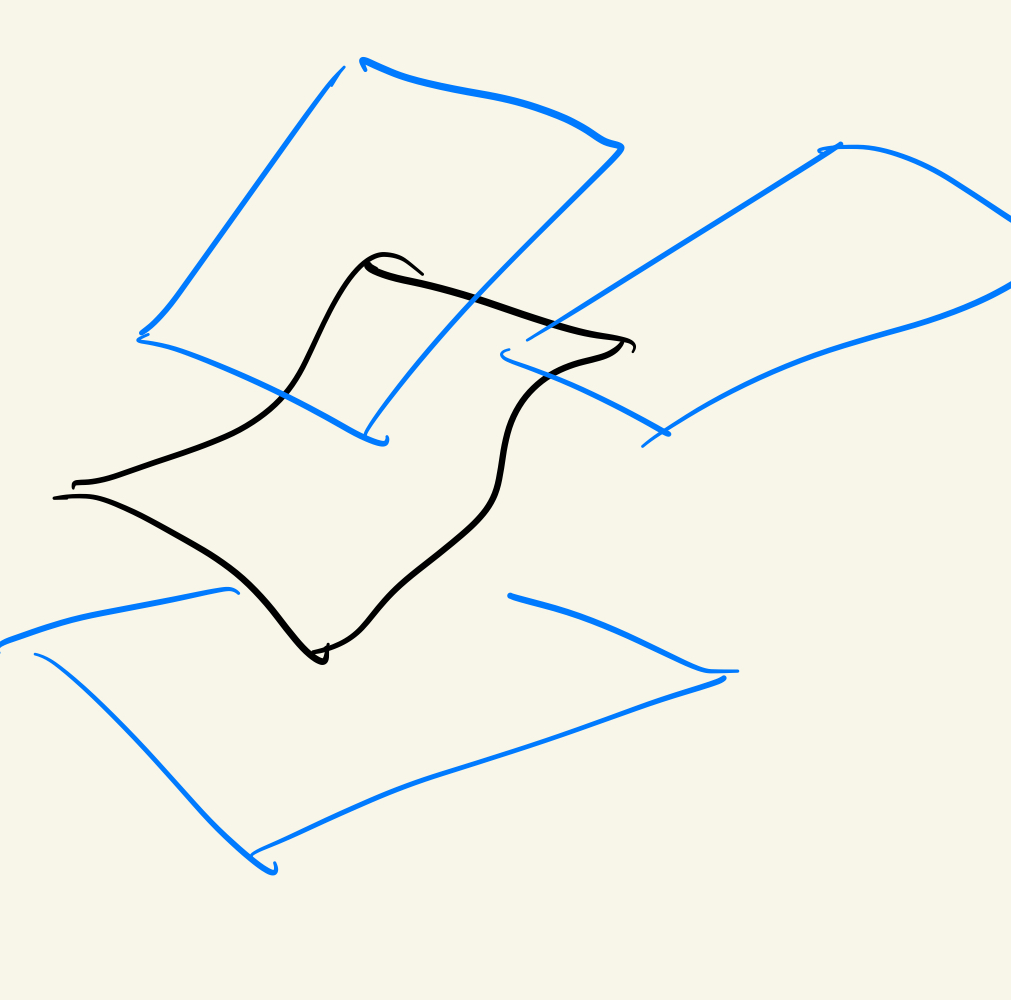
\includegraphics[width=0.3\textwidth]{fig1}
	\caption*{Riemann surfaces case}
\end{figure}
\begin{quotation}
A line bundle on a riemann surface is like its tangent bundle--a bunch of planes put somehow over the points of the surface. And a section is like a vector field. And the zeroes of the section are a bunch points. So the submanifold is a bunch of points.
\end{quotation}



\subsubsection*{ampleness in Hartshorne}

Here's the \textbf{upshot} about ampleness:

From II.7, subsection \textit{Ample Invertible Sheaves}, p. 153:
\begin{quotation}
	Now that we have seen that a morphism of a scheme \(X\) to a projective space can be characterized by giving an invertible sheaf on \(X\) and a suitable set of its global sections, […]

	Recall that in §5 we defined a sheaf \(\mathcal{L}\) on \(X\) to be \textit{\textbf{very ample relative to \(Y\)}} if there is an immersion \(i: X \to \mathbb{P}^n_Y\) for some \(n\) such that \(\mathcal{L} \cong i^*\mathcal{O}(1)\). In case \(Y = \operatorname{Spec}A\), this is the same thing as saying that \(\mathcal{L}\) admists a set of global sections \(s_0,\ldots,s_n\) such that the corresponding morphism \(X \to \mathbb{P}^n_A\) is an immersion.

	We have also seen (5.17) that if \(\mathcal{L}\) is a very ample invertible sheaf on a projective scheme \(X\) over a noetherian ring \(A\), then for any coherent sheaf \(\mathcal{F}\) on \(X\), there is an integer \(n_0>0\) such that for all \(n \geq  n-\), \(\mathcal{F} \otimes \mathcal{L}^n\) is generated by global sections. […]
	\begin{defn}\leavevmode
	An invertible sheaf \(\mathcal{L}\) on a noetherian scheme \(X\) is said to be \textit{\textbf{ample}} if for every coherent sheaf  \(\mathcal{F}\) on \(X\) there is an integer \(n_0>0\) (depending on \(\mathcal{F}\)) such that for every \(n \geq  n_0\) the sheaf \(\mathcal{F} \otimes \mathcal{L}^n\) is generated by its global sections. (Here \(\mathcal{L}^n:= \mathcal{L}^{\otimes n}\).)
	\end{defn}
	[…]
	\begin{thing5}{Remark II.7.4.3}\label{rk:II.7.4.3}\leavevmode
		[…] we will see below (7.6) that if \(\mathcal{L}\) is ample, then some tensor power  \(\mathcal{L}^m\) of \(\mathcal{L}\) is very ample.
	\end{thing5}
\end{quotation}

So, being very ample is just a term to hide the possibility of embedding the variety in a projective space and pulling back the hyperplane bundle to that line bundle. But it turns out that this is equivalent to being generated by global sections in some sense (maybe taking tensor product).

\begin{thing4}{Example II.6.4}\label{exer:}\leavevmode
	We will see later (IV, 3.3) that if  \(D\) is a divisor on a complete nonsingular curve \(X\), them \(\mathcal{L}(D)\) is ample iff \(\operatorname{deg}D>0\). This is a consequence of the Rimeann-Roch theorem.
\end{thing4}

\begin{question}\leavevmode
What's up with the base-points?
\end{question}

To answer we move along to subsection  \textit{Linear systems} in Hartshorne.
\begin{quotation}
	[…] global sections of an invertible sheaf correspond to effective divisors on a variety. Thus giving an invertibnle sheaf and a set of its global sections {\color{6}(which is related to finding the embedding of the variety into projective space pulling back the hyperplane bundle!)} is the same as giving a certain set of effective divisors, all linearly equivalent to each other.
\end{quotation}

\begin{thing6}{Idea}[dani]\leavevmode
That we can associate divisors to sections. Then we consider all linearly equivalent divisors to a given one (a linear system), which corresponds to a set of sections \(V \subseteq \Gamma(X,\mathcal{L})\).
\end{thing6}

\textbf{And then} 
\begin{thing4}{Lemma II.7.8}\label{lem:II.7.8}\leavevmode
	[…] In particular, [a linear system] \(\mathfrak{d}\) is base-point-free iff \(\mathcal{L}\) is generated by the global sections in \(V\).
\end{thing4}
\subsection{line systems}
\begin{itemize}
  \item A \textbf{line system} is the set of effective divisors associated to sections of a line bundle. How? Every section defines an effective divisor given by its zero-locus.
  
  \item \textbf{Definition:} An \emph{effective divisor} is a finite formal sum of points (or subvarieties of codimension 1) with nonnegative integer coefficients:
  \[
  D = \sum n_i p_i, \quad n_i \geq 0
  \]
  
  \item \textbf{Claim:} The zero-locus of a section is an \emph{effective} divisor.
\item \textbf{Claim:} The zero-locus of a section is a codimension-1 subvariety. 

  \item \textbf{Claim:} Two proportional sections give the same effective divisor. (So that's why the linear system is the projectivization of the space of sections — for every section we consider all its proportional sections.)
\item \textbf{Claim:} The associated line bundle to any element of a linear system (associated to a given line bundle \(L\)) is \(L\). 
\end{itemize}

\textbf{Conclusion:} The line system is the projectivization of the space of sections.

\textbf{Epiphany:} The canonical map associated to a very ample line bundle is an embedding of \( X \) into… its linear system?
\subsection{bertini theorem}

\begin{thing6}{bertini theorem}[\cite{gri}, p.137]\leavevmode
The generic element of a linear system is smooth away from the base locus of the system.
\end{thing6}

and that finally. makes. sense. Because a linear system is the projectivized space of smooth sections, which says nothing, nothing at all, but now I know: a section has a zero locus, and proportional sections give the same zero locus (that's why the linear system is defined as a projectivization) and that zero locus is what we want to define as a smooth submanifold in complex world because there is no regular value theorem because all functions are constant so BERTINI IS REGULAR VALUE THOREM VERSION FOR COMPLEX GEOMETRY.

\begin{proof}\leavevmode

\end{proof}

Here's Telegram messages:

One of the weakest forms that I needed in order to make some sense of Lefschetz hyperplane theorem is the following:

Let \(X\) in \(\mathbb{P}^N\) be a smooth variety.

Then for generic hyperplane H the hyperplane section
\[X_H=X \cap H\]
is smooth.

I also formulated another version of Bertini's Theorem, often used by algebraic geometers, which involves a few more definitions (from the section on divisors and line bundles).

Let \( X \) be an algebraic variety (not necessarily projective or compact).

On \( X \), we consider a \emph{linear system} (of divisors). We define the \emph{fixed components} of a linear system to be a divisor that is the minimum (in the sense of divisors) over all representatives in the system. A linear system is called \emph{movable} if it has no fixed components. Any linear system can be decomposed into a sum of a fixed component and a movable linear system, known as the \emph{movable part}.

The \emph{base locus} of a linear system is defined as the base locus of its movable part. For a movable linear system of divisors, the base locus is the intersection of all divisors in the system. In other words, it is the indeterminacy locus of the rational map to projective space defined by the given linear system. We denote the base locus by \( \operatorname{Bs}(L) \) or \( \operatorname{Bs}(|H|) \), etc.

\begin{thm}[Bertini]
Let \( X \) be an algebraic variety over a field of characteristic 0, and let \( |H| \) be a movable linear system on \( X \). Then, for a generic divisor \( H \in |H| \), its singularities are contained in the union of \( \operatorname{Sing}(X) \) and \( \operatorname{Bs}(|H|) \).
\end{thm}

\begin{exercise}
Can you derive this version of Bertini’s Theorem from the special case of the theorem for pencils?
\end{exercise}




\subsection{adjunction formula}

\subsubsection{Sergey}

\begin{quotation}
	Today evening (17h) we discussed the \emph{adjunction formula}, written sometimes as 
\[ K_D = K_X + D \quad \text{or} \quad K_Y = (K_X + Y)|_Y. \]

The formulation and proof are relatively straightforward for smooth hypersurfaces in smooth total spaces (manifold case). Some objects featured in the discussion include: tangent or cotangent bundles, conormal sheaf or normal bundle, and determinants of vector bundles.

We also discussed how to define determinants for complexes of vector bundles, and how to define determinants of coherent sheaves on smooth projective varieties by taking their resolution. More generally, the determinant is well-defined for objects of the bounded derived category of vector bundles, and behaves well in triangles.

This all follows from the formula for determinants of finite-dimensional vector spaces in a short exact sequence:
\[
0 \longrightarrow U \longrightarrow V \longrightarrow W \longrightarrow 0
\]
In this case, we have a canonical isomorphism:
\[
\det(V) \cong \det(U) \otimes \det(W),
\]
and there is a quite explicit canonical isomorphism. Thanks to its canonicity, it globalizes to trivial vector bundles, and locally trivial vector bundles (so to all vector bundles), and then by standard homological algebra and $K$-theory to complexes of vector bundles.

In fact, the same standard $K$-theory argument shows that the isomorphism class of $\det(C)$ in $\mathrm{Pic}(X)$ depends only on the class $[C]$ of the complex in the $K$-group $K(X)$.

\medskip

\noindent One thing we have not (yet) discussed is how to prove that $N \cong \mathcal{O}(D)$.

More generally, we looked at the relation between the (co)normal sheaf $\mathcal{N}_{X/Y}$ and the ideal sheaf $\mathcal{I}_Y$.

\medskip

\noindent \textbf{Hint:} the conormal sheaf is isomorphic to
\[
\mathcal{I}_Y / \mathcal{I}_Y^2.
\]
From this relation, the formula $N = \mathcal{O}_X(D)$ follows easily.
\end{quotation}

\begin{exercise}[dani puts this on April 8 2025]\leavevmode
Show that canonical isomorphism of determinant bundles given an exact sequence. \textbf{Solution at MSE:} \href{https://math.stackexchange.com/questions/822470/exterior-power-commutes-with-direct-sum}{here}.
\end{exercise}

\subsubsection{Huybrechts}
\iffalse

\begin{thing4}{Definition 2.2.16}[\cite{huc}]\label{def:2.2.16}\leavevmode
Let \(Y \subset X\) be a complex submanifold. The \textit{\textbf{normal bundle}} of \(Y\) in \(X\) is the holomorphic vector bundle \(\mathcal{N}_{Y/X}\) on \(Y\) is the cokernel of the natural injection \(\mathcal{T}_Y \subset \mathcal{T}_X|_{Y}\). Thus there exists a short exact sequence of holomorphic vector bundles, the \textit{\textbf{normal bundle sequence}}:
\[\begin{tikzcd}0\arrow[r]&\mathcal{T}_Y\arrow[r]&\mathcal{T}_X|_{Y}\arrow[r]&\mathcal{N}_{Y/X}\arrow[r]&0\end{tikzcd}\]
\end{thing4}

\begin{thing7}{Explanation}[Example 2.23, \cite{lec}]\leavevmode
The \textit{\textbf{holomorphic normal bundle}} of \(Y\) in \(X\) is the bundle \(NY \to Y\) defined by \(NY:=(T'X|_{Y}/T'Y\) where the apostrophe means holomorphic tangent bundle for Lee. So probably this is the metric-free definition of the normal bundle.  ``(It is important to observe that the \textit{\textbf{geometric normal bundle}} that can be defined as the set of tangent vectors that are orthogonal to \(S\) with respect to some Riemannian metric on \(M\) will not in general have holomorphic transition functions.)" So maybe metric normal bundle may not be holomorphic, and instead metric-free normal bundle is holomorphic always?
\end{thing7}

\begin{thing6}{Dream}\leavevmode
It'd still be nice to understand the construction geometrically: take the tangent bundle of the ambient variety, and quotient by the tangent bundle of the subvariety. At a point, we have collapsed the tangent bundle of the subvariety, and all we are left with is the vectors that are not tangent to the subvariety. I guess it kind of makes sense: take for example a curve on \(\mathbb{R}^3\), collapse the tangent line at a point of the curve, and you get \(\mathbb{R}^2\).
\end{thing6}
\fi
So what is the determinant bundle? See basic math section, but it is the top exterior power of the bundle, i.e. at every point you just put the top exterior power of the corresponding vector space.

\begin{thing4}{Proposition 2.2.17, \cite{huc}}[Adjunction formula]\label{prop:2.2.17}\leavevmode
Let \(Y\) be a submanifold of a complex manifold \(X\). Then the canonical bundle \(K_Y\) of \(Y\) is naturally isomorphic to the line bundle \(K_X|_{Y} \otimes \det(\mathcal{N}_{Y/X})\).
\end{thing4}

\begin{proof}\leavevmode
So you see, the proof is that exercise of the last section.
\end{proof}

There's more. Today I asked Bruno well how do you associate a divisor to a section of a line bundle? \textit{It's the zeros of the section!} Now think of the normal bundle of the divisor. What is it?
\begin{thing4}{Proposition 2.4.7}[\cite{huc}]\label{prop:2.4.7}\leavevmode
Let \(X\) be a smooth hypersurface of a complex manifold \(Y\) defined by a section \(s \in H^{0}(Y,L)\) of some holomorphic line bundle \(L\) on \(Y\). Then \(\mathcal{N}_{X/Y}\cong L_X\) and thus 
\end{thing4}

How to think this?

\begin{figure}[H]
	\centering
	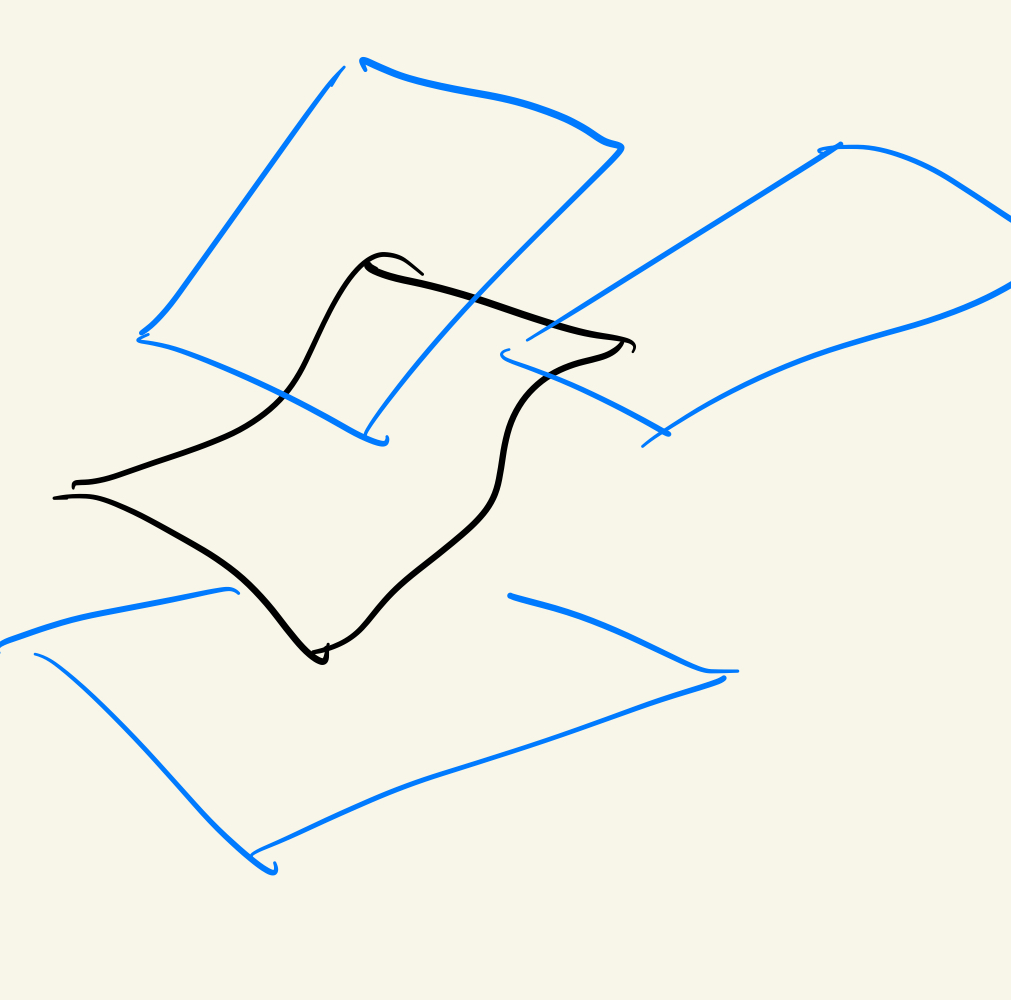
\includegraphics[width=0.4\textwidth]{fig1}
	\caption*{Riemann surfaces case}
\end{figure}
 \begin{quotation}
 	So take that Riemann surface and that line bundle and that section of that line bundle and that zero locus of that section of that line bundle on that Riemann surface, which is your divisor/submanifold. It's some points, just some points. The tangent space of some points is totally boring, it's some points again, so the normal space is all the space of the ambient manifold, so the line bundle again. Whoa.
 \end{quotation}

 \begin{thing7}{proposition finishes:}\leavevmode
 and thus \(K_X \cong (K_Y \otimes L)|_{X}\).
 \end{thing7}

 \begin{upshot}\leavevmode
 I think the proof is essentially the canonical isomorphism of determinant sheaves of the normal exact sequence.
 \end{upshot}

\subsubsection{a formula from Hartshorne}

This is really an application of Riemann-Roch for surfaces:

\begin{thing1}{Proposition V.1.5}[\cite{hart}]\leavevmode
If \(C\) is a nonsingular curve of genus \(g\) on the surface \(X\) and \(K\) is the canonical divisor on \(X\), then
\[2g-2=C.(C+K).\]

\end{thing1}

\subsubsection{Kodaira ampleness criterion}

In K3 lecture 9 we have

\begin{thm}[Kodaira]\leavevmode
A bundle \(L\) is very ample iff \(c_1(L)\) is a Kähler class.
\end{thm}

\begin{thing7}{Recall}\leavevmode
that a line bundle is \textit{\textbf{prequantizable}} if its curvature is symplectic and integral.
\end{thing7}

\subsection{serre duality}
\begin{thing6}{serre duality}[II.5.32\cite{voi}]\label{thm:5.32}\leavevmode
The pairing
\[H^{q}(X,\mathcal{E})\otimes H^{n-q}(X,\mathcal{E}^*\otimes K_X)\to H^{n}(X,K_X)\cong\mathbb{C}\]
(probably given by some integral) between
\[H^{q}(X,\mathcal{E})\qquad \text{and} \qquad H^{n-q}(X,\mathcal{E}^* \otimes K_X)\]
is perfect.
\end{thing6}
So when you put the dual \(\vee\) on one of these you get isomorphism.


\begin{thing6}{Serre duality}[dani notes Complex geometry course 2024.1]\leavevmode
\[H^{k}(X,\mathcal{L})^{\vee}=H^{n-k}(X,\omega_X \otimes \mathcal{L}^*)\]
\end{thing6}

\subsection{kodaira vanishing}
…``based on the following special case of the Kodaira-Akizuki-Nakano vanishing theorem":
\begin{thing6}{kodaira vanishing}[thm. 7.13 \cite{voi}]\label{thm:kodaira vanishing}\leavevmode
	Let \(L\) be a positive holomorphic line bundle over a compact complex manifold. Then for every \(q>0\), we have
	\[\boxed{H^{q}(X,K_X \otimes \mathcal{L})=0}\]
\end{thing6}

From Telegram:

\begin{quotation}
	``S, [19 Jun 2024 13:31:41]:
Useful formulation, maybe a most used one

\[H^q(K+ample) = 0 \qquad \text{ for}\qquad  q>0\]

in particular

\[H^1(X,K+D) = 0\] if \(D\) is ample (or positive, which is the same, but in the proof we only used positiveness).



trick: if you want to prove some vanishing of some line bundle, rewrite your line bundle as K+something, then check if you can make this something ample."
\end{quotation}

\subsection{Positive \((1,1)\)-forms}
Any positive \((1,1)\) form looks like this: \(\sum \alpha I x_i \wedge x_i\) for some positive functions \(\alpha_i \geq 0\).

\subsection{Hodge Index Theorem}

\begin{thing4}{Theorem V.1.9}[Hodge Index Theorem]\label{prop:V.1.9}\leavevmode
Let
\end{thing4}


\subsection{Kähler metric}
The Kähler form is the differential of a plurisubharmonic function \(\psi\). that is \(\omega=d d^c \psi=\sqrt{-1} \partial \partial \psi\).

\subsection{Picard group, Neron-Severi group}

\begin{defn}[dani]\leavevmode
\textit{\textbf{Picard group}} is the group of line bundles with tensor product.
\end{defn}

\begin{remark}\leavevmode
See \cite{hart} p. 151 for the quick comment ``We have seen (6.17) that \(\operatorname{Pic}\mathbb{P}^n_k \cong\mathbb{Z}\) and is generated by \(\mathcal{O}(1)\)".
\end{remark}

\begin{thing4}{Definition}[\cite{huk}, p.5]\leavevmode
\textit{\textbf{Néron-Severy group}} of an algebraic surface \(X\) is the quotient
\[\operatorname{NS}(X):=\operatorname{Pic}(X) /\operatorname{Pic}_0(X)\]
by the connected component of the Picard variety \(\operatorname{Pic}(X)\), i.e. by the subgroup of line bundles that are \textit{algebraically} equivalent to zero (?).
\end{thing4}

\begin{thing4}{Definition}[\cite{huk}, p.5]\label{prop:}\leavevmode
\[\operatorname{Num}(X):=\operatorname{Pic}(X)/\operatorname{Pic}^\tau(X)\]
where \(\operatorname{Pic}^\tau(X)\) is the subgroup of \textit{numerically trivial} line bundles, i.e. line bundles \(L\) such that \((L.L')=0\) for all line bundles \(L'\). (E.g. any  \(L \in \operatorname{Pic}^0\) is numerically trivial.) 
\end{thing4}

\subsection{K3 surfaces}
\begin{defn}[dani]\leavevmode
A \textit{\textbf{K3}} surface is a complex surface with trivial canonical bundle and vanishing first (co)homology. (It's dimension 2 so 1st cohomology is first homology by Poincaré.)
\end{defn}

\begin{defn}[K3 course]\leavevmode
A \textit{\textbf{K3 surface}} is a complex surface \(M\) with \(b_1=0\) (Betti number is dimension of homology) and \(c_1(M,\mathbb{Z})=0\). Recall that the Chern class coming from the exponential sequence is \(\operatorname{Pic}(M) \xrightarrow{c_1}H^{2}(M,\mathbb{Z})\), so in particular it means that the first Chern class of the canonical bundle \(K_X \in \operatorname{Pic}(M)\) is trivial, which in turn makes it trivial via Hodge theory.
\end{defn}

\begin{remark}\leavevmode
\cite{huk} shows that K3 surfaces have trivial (algebraic) fundamental group (what is that?) in remark 2.3.
\end{remark}

\begin{defn}[\cite{huk}]\leavevmode
A \textit{\textbf{K3 surface}} over \(k\) is a complete non-singular variety \(X\) of dimension two such that
 \[\Omega^2_{X/k}\cong \mathcal{O}_X\qquad \text{and} \qquad H^{1}(X,\mathcal{O}_X)=0\]
\end{defn}

\begin{thing4}{Proposition 1.2.1}[\cite{huk}]\leavevmode
\(\operatorname{NS}(X)\) and its quotient  \(\operatorname{Num}(X)\) are finitely generated.

The rank of \(\operatorname{NS}(X)\) is called the \textit{\textbf{Picard number}} \(\rho(X):=\operatorname{rk}\operatorname{NS}(X)\).
\end{thing4}

\begin{thing4}{Proposition 1.2.4}[\cite{huk}]\label{prop:1.2.4}\leavevmode
For a K3 surface \(X\) the natural surjections are isomorphisms (\textbf{warning:} the second isomorphism might not hold for general complex K3 surfaces):
\[\operatorname{Pic}(X) \xrightarrow{\sim}\operatorname{NS}(X)\xrightarrow{\sim}\operatorname{Num}(X)\]
and the intersection pairing on \(\operatorname{Pic}(X)\) is even, non-degenerate, and of signature \((1,\rho(X)-1)\).
\end{thing4}

\begin{remark}[\(\chi(\text{K3},\mathcal{O}_X)=2\)]\leavevmode
From \cite{huk} I.2.3, p.6:
\begin{quotation}
	``For a K3 surface \(X\) one has by definition \(h^{0}(X,\mathcal{O}_X)=1\) and \(h^{1}(X,O_X)=0\). Moreover, by Serre duality \(H^{2}(X,\mathcal{O}_X)\cong H^{0}(X,\omega_X)^*\) and hence \(h^{2}(X,\mathcal{O}_X)=1\). Therefore,
	\[\chi(X,\mathcal{O}_X)=2."\]
\end{quotation}
So here's that computation using Serre duality:
\begin{align*}
H^{0}(X,\mathcal{O}_X)&\overset{\substack{\text{Serre}  \\ \text{duality} } }{=}H^{2}(X,\mathcal{O}_X^*\otimes K_X)^* \overset{\substack{\text{dual}  \\ \text{of trivial} \\ \text{is the}\\\text{trivial} }}{=}H^{2}(X,\mathcal{O}_X \otimes K_X)^* \overset{\substack{\text{you are}  \\ \text{a K3} } }{=}H^{2}(X,\mathcal{O}_X)^*=\mathbb{C}^*=\mathbb{C}
\end{align*}
because the dual.
\end{remark}

\begin{thing7}{don't get confused}\leavevmode
Here's three things that are not the same:
\begin{enumerate}
\item \(\chi(X,\mathcal{O}_X)\), the Euler characteristic of the structure sheaf \(\mathcal{O}_X\).
\item \(\chi(X)\), the Euler characteristic of a manifold. Probably \(\sum (-1)^i \dim H_{i}(X,\mathbb{Z})\).
\item \(\chi(X,K_X)\), the Euler characteristic of the line bundle \(K_X\), because bundles have Euler characterstic too.
\end{enumerate}
\end{thing7}

\subsubsection{Kummer}

Take a complex 2-torus \(A\) and consider the involution \(\tau:[z_1,z_2]\mapsto -[z_1,z_2]\). It has 16 fixed points, so the quotient \(A/\tau\) has singularities. Smooth it to obtain \(\hat{A}\) and consider the involution \(\hat{\tau}\). Then \(\hat{A}/\hat{\tau}\) is a K3.

\subsection{Fubini-Study}
It's a metric, it's a symplectic form. \textit{\textbf{Fubini-Study (symplectic) form}} is a closed 2-form defined on \(\mathbb{C}P^{n}\) as the exterior differential of the logarithm of the length functions \(\ell=\sum |z_i|^2\), i.e. \(\omega=dd^c \operatorname{log} \ell\).

This also has a local expression in coordinates \((z_1,\ldots,z_n)\) that might be interesting.

The \textit{\textbf{Fubini-Study metric}} is \(g(\cdot ,\cdot )=\omega(\cdot ,I\cdot )\).

\subsection{hypercomplex manifolds}

\begin{defn}\leavevmode
	A manifold $M$ is \textit{\textbf{hypercomplex}} if it has three integrable almost complex structures  $I$,  $J$, $K$ satisfying the quaternionic relations $I^2=J^2=K^2=-\operatorname{Id}$ and $I J=-J I=K$.
\end{defn}

\subsubsection{Obata connection}

\begin{remark}[Obata Connection, GPT]
    Given a hypercomplex manifold $(M, I, J, K)$, there exists a unique torsion-free connection $\nabla^{\operatorname{ob}}$ such that
    \[
    \nabla^{\operatorname{ob}} I = \nabla^{\operatorname{ob}} J = \nabla^{\operatorname{ob}} K = 0.
    \]
    This is called the \textit{Obata connection}. Unlike the Levi-Civita connection, it is not necessarily compatible with a metric. Instead, it preserves the entire hypercomplex structure and serves as the natural connection in hypercomplex geometry.
\end{remark}

\subsubsection{\(\mathsf{SU}(n)\)}

\textbf{How to think of \(\mathsf{SU}(2)\)} Take a real vector space \(V\) equipped with a hypercomplex structure and think of \(\mathsf{SU}(2)\) as
\[\mathsf{SU}(2)=\{a+b I+c J+ d K: a^2+b^2+c^2+d^2=1,\qquad a,b,c,d \in \mathbb{R} \}\]
Just because that's the way to go. (But at some point of terrenal mathematics you should prove that indeed, \(\mathsf{SU}(2)\cong \text{unit quaternions} \cong S^3\).)

But what's the lance?
\begin{quotation}
	``We are using these three complex structures (quaternionic is the term right? (it's not: this is called a \textit{\textbf{hypercomplex structure}}) for their nice relations IJ=-JI=K) to \textit{model} the division algebra H that is god-given. Then this thing which is a group \textit{acts} on the space of endomorphisms of the quaternionic vector space by conjugation"

	\vspace{1em}
	\hfill Yes---you're getting it beautifully now.
\end{quotation}


\subsection{Fano}

\begin{exercise}\leavevmode
By Kodaira vanishing theorem, you can show that the cohomology \(H^{i}(X,L)\) of a Fano variety \(X\) vanishes. You just have to put \(L=\mathcal{O}(k)\) with \(k\geq  -r\) for the \textit{\textbf{Fano index}} 
\[r(X)=\operatorname{min}\{r:\frac{c_1(X)}{r}\in H^{2}(X,\mathbb{Z})\}.\]
Anyway the point is that \(\operatorname{Pic}(X)\cong H^{2}(X,\mathbb{Z})\) for Fano.
\end{exercise}

\section{complex analysis}

\subsection{cauchy-riemann}

\(f:U \subset \mathbb{C} \to \mathbb{C}\) is \textit{\textbf{holomorphic}} at \(z_0\in U\) if
\[\lim_{z \to z_0} \frac{f(z_0-z)-f(z_0)}{z-z_0}\]
exists. And also, don't get confused, \(h\in \mathbb{C}\),
\[\lim_{h \to 0} \frac{f(z_0+h)-f(z_0)}{h}\]

\begin{thing7}{Cauchy-Riemann}\leavevmode
The idea is to use the second definition along the \(x\) axis, call \(f=u+iv\) and  \(z_0=x_0+iy_0\). To take derivative along the \(x\) axis you take \(h\) and don't get confused, this time \(h\) \textit{is} just a real number
\begin{align*}f(z_0+h)-f(z_0)&=\Big(u(x_0+h,y_0)+iv(x_0+h,y_0)\Big)-\Big(u(x_0,y_0)+iv(x_0,y_0)\Big)\\
&=\Big(u(x_0+h,y_0)-u(x_0,y_0)\Big)+i\Big(v(x_0+h,y_0)-v(x_0,y_0)\Big)
\end{align*}
which will give you upon limiting:
\[\frac{\partial u}{\partial x}+i\frac{\partial v}{\partial x}\]
Do the other one, probably you'll get
\[\frac{\partial v}{\partial y}-i\frac{\partial u}{\partial y}\]
But do do it. The trick is that again, don't get confused, \(h\) is real but you put \(i\):
\begin{align*}
f(z_0+ih)-f(z_0)&=\Big(u(x_0,y+ih)+iv(x,y+ih)\Big)-\Big(u(x,y)+iv(x,y)\Big)\\
&=\Big(u(x,y+ih)-u(x,y)\Big)+i\Big((v(x,y+ih)-v(x,y)\Big)\ldots
\end{align*}
And looks the same but actually you quotient by… \(ih\):
\begin{align*}\frac{f(z+ih)-f(z)}{ih}&=\frac{1}{i}\left(\frac{\partial u}{\partial y}+i\frac{\partial v}{\partial y}\right)=\frac{\partial v}{\partial y}-i\frac{\partial u}{\partial y}
	\end{align*}
Aha! Right so real with real and imaginary-imaginary,
\[\frac{\partial u}{\partial x}=\frac{\partial v}{\partial y},\qquad \frac{\partial v}{\partial x}=-\frac{\partial u}{\partial y}\]
\end{thing7}




\bibliography{bib.bib}

\end{document}
